\documentclass[aps,preprint,nofootinbib,floatfix]{revtex4-1}
%\documentclass{article}

%\usepackage{nips_2017}

% to compile a camera-ready version, add the [final] option, e.g.:
%\usepackage[final]{nips_2017}

%\usepackage{nicefrac}       % compact symbols for 1/2, etc.
%\usepackage{microtype}      % microtypography
\usepackage{amsmath,amssymb,amsfonts,amsthm,amscd,bm,bbm}
%\usepackage{mathtools}
%\usepackage{printlen}
\usepackage[inline]{enumitem}
%\usepackage{cite}
%\usepackage{bbm}

\usepackage[pdftex]{graphicx}
\graphicspath{{./figs/}}

\usepackage{algorithmic}
\usepackage{algorithm}
\usepackage[none]{hyphenat}
\usepackage{multirow}
\usepackage{colortbl}
\usepackage{array,booktabs}
\usepackage{xcolor}
\usepackage{makecell}

\hyphenation{op-tical net-works semi-conduc-tor}

\newtheorem{theorem}{Theorem}
\newtheorem{definition}[theorem]{Definition}
\newtheorem{assumption}[theorem]{Assumption}
\newtheorem{lemma}[theorem]{Lemma}
\newtheorem{corollary}[theorem]{Corollary}
\newtheorem{proposition}[theorem]{Proposition}
\newtheorem{conjecture}[theorem]{Conjecture}
\newtheorem{remark}[theorem]{Remark}
\newtheorem{example}{Example}

%% our definitions %%%%%%%%%%%%%%%%%%%%%%%%%%%%%%%%%%%%%%%%%%%%%%%%%%%%%%%%%%%%
\DeclareMathOperator{\aff}{aff}
\DeclareMathOperator{\st}{s.t.}
\DeclareMathOperator{\LC}{LC}
\DeclareMathOperator{\affnot}{aff_0}
\DeclareMathOperator{\conv}{conv}
\DeclareMathOperator{\relint}{relint}
\DeclareMathOperator{\vol}{vol}
\DeclareMathOperator{\range}{range}
\DeclareMathOperator{\image}{im}
\DeclareMathOperator{\nullspace}{null}
\DeclareMathOperator{\area}{area}
\DeclareMathOperator{\vspan}{span}
\DeclareMathOperator{\id}{Id}
\DeclareMathOperator{\cond}{cond}
\DeclareMathOperator{\prox}{prox}
\DeclareMathOperator*{\argmax}{arg\,max}
\DeclareMathOperator*{\argmin}{arg\,min}
\DeclareMathOperator*{\minimize}{minimize}
\DeclareMathOperator{\diag}{diag}
\DeclareMathOperator{\Tr}{Tr}

\newcommand\Energy{\mathcal{E}}
\newcommand\E{\mathbb{E}}
\newcommand\kk{K}
\newcommand\kkk{h}
\newcommand\Hk{{\mathcal{H}}_{\kk}}
\newcommand\HH{\mathcal{H}}
\newcommand\C{{\mathcal{C}}}
\newcommand\OO{{\mathcal{O}}}
%\newcommand\Zt{\widetilde{Z}}
\newcommand\Zt{Y}
%\newcommand{\Ind}[1]{\delta_{#1}}
\newcommand{\Ind}[1]{\mathbbm{1}_{#1}}
\newcommand\e{e}
\newcommand\om{\omega}


\begin{document}


\title{Nonparametric Clustering from  Energy Statistics}

\author{Guilherme Fran\c ca}
\email{guifranca@gmail.com} 
%\affiliation{Johns Hopkins University}

\author{Joshua T. Vogelstein}
\email{jovo@jhu.edu}

\affiliation{Johns Hopkins University}


\begin{abstract}
Energy statistics 
was proposed by 
Sz\' ekely in the 80's
inspired by the Newtonian gravitational potential from classical mechanics,
and it provides a nonparametric test for equality of distributions.
It was generalized to 
metric spaces of strong negative type,
and more recently a connection with reproducing kernel Hilbert spaces 
was proposed.
%Although  
%extensively used in statistics, it
%has not been previously incorporated in machine learning problems.
% @gui: not sure what you mean?  what counts as machine learning?  be specific, i think yo mean clustering?  even then, it is not true, both the master's thesis and the RKHS paper kind of do it.  be as general as possible about the gap that we are filling, but not more general
% @jovo: I think we should just remove the phrase. 
Here we consider the problem of clustering data from
an energy statistics theory perspective.
We provide a precise mathematical formulation yielding
a quadratically constrained quadratic program (QCQP), which we show
to be equivalent
to kernel $k$-means optimization problem.
Thus, our results imply a first principles derivation of 
kernel $k$-means from energy statistics.
% @gui: have other people shown a relationship between kernel k-means and say, RKHS, or something else? 
% @jovo: yes, any kernel method is defined on a HKHS. 
% For instance ref [11] is the first one to consider kernel k-means in a 
% RKHS. The whole problem is how do you formulate a 
% statistical problem in a RKHS. In the case of
% energy this was done only by [6], and it's based on this work that we 
% have the theory presented in this paper
Moreover, we also consider a weighted version of energy statistics 
applied to clustering, which makes connection to 
graph partitioning problems.
To find local optimizers of such QCQP we consider an iterative
algorithm based on Hartigan's method, which in this case
has the same computational cost 
as kernel $k$-means algorithm but usually with better clustering
quality. We provide carefully designed numerical experiments
showing the superiority of this method compared to
kernel $k$-means, standard $k$-means, and gaussian mixture models.
\end{abstract}

\maketitle

%%%%%%%%%%%%%%%%%%%%%%%%%%%%%%%%%%%%%%%%%%%%%%%%%%%%%%%%%%%%%%%%%%%%%%%%%%%%%%%
\section{Introduction}

Energy statistics \cite{Szkely2013}
is based on a 
notion of statistical potential energy between probability distributions,
in close analogy to Newton's gravitational
potential in classical mechanics. 
It provides a nonparametric test for equality of distribution which
is achieved under minimum energy. When probability distributions
are different, this statistical potential 
energy diverges as sample size increases.
Energy statistics has been applied to several goodness-of-fit 
hypothesis tests, 
multi-sample tests of equality of distributions, analysis of variance
\cite{RizzoVariance}, nonlinear
dependence tests through
distance covariance and distance correlation, which generalizes the Pearson
correlation coefficient, and  
hierarchical clustering \cite{RizzoClustering} by extending Ward's
method of minimum variance. We refer to \cite{Szkely2013} and 
references therein for an overview.
Moreover, an energy statistics formulation
to clustering was already proposed in \cite{Kgroups} 
which greatly motivated this paper.

Recently, distance covariance was 
generalized from Euclidean
spaces to metric spaces of strong negative type \cite{Lyons}.
Furthermore, a unifying framework establishing an equivalence
between generalized energy distances to maximum
mean discrepancies (MMD), which are distances between embeddings of
distributions in reproducing kernel Hilbert spaces (RKHS), was
established \cite{Sejdinovic2013}. This provides the 
link between concepts used in energy statistics and concepts
commonly used in machine learning, and form the basis of our approach.

The clustering problem has a long history in machine learning.
Perhaps the most used method is $k$-means \cite{Lloyd,MacQueen,Forgy}, which
is based on Lloyd's heuristic \cite{Lloyd} of assigning a data point to
the cluster with closest center. The only statistical 
information about each cluster
comes from its mean and it is thus sensitive to outliers.
% @gui: algorithms don't make assumptions, theorems do.  also, algorithms cannot be parametric or non-parametric, that is a property only of the statistical model, or an estimator. 
%Moreover, $k$-means
%is strongly parametric, assuming that data is isotropically and normally
%distributed since it is a special case of gaussian mixture models (GMM) 
% @gui: k-means is NOT a special case of GMM, GMM is a soft clustering (not fuzzy, in stats and machine learning we don't say "fuzzy"), where as k-means is a hard clustering.  k-means is certainly closely related to GMM though.
%through the expectation maximization (EM) algorithm. 
Nevertheless,
$k$-means works very well when data is linearly separable 
in Euclidean space.
%, with a clear resolution of cluster centers and without
%significant overlap of the points belonging to different clusters.
% @gui:  don't know what "clear resolution of cluster centers" adds to this?
% @jovo: commented out some parts above and included new phrase here.
Gaussian mixture models (GMM) is also very commonly used for 
clustering,
however it is strongly parametric, as $k$-means which is closely related.

To account for nonlinearities, kernel methods were introduced 
\cite{Smola,Girolami}. A mercer kernel \cite{Mercer} is used to implicitly
map data points to a RKHS, then clustering can be performed in the associated
Hilbert
space by using its inner product. 
%This enables one to cluster way more complicated datasets, 
This enables one to cluster data that is not separable in Euclidean space.
% @gui: algorithms cluster, doesn't matter how complicated the data are.  so, what do you actually mean here?  perform well empirically? what does "complicated" actually mean?
% @jovo: what I mean is not tied to any algorithm. I want to say that kernel
% methods allows one to cluster data that is not separable in Euclidean space.
% I modified the phrase, see if it's better
However, the kernel choice remains the biggest challenge
since there is no principled theory to construct a kernel for a given dataset,
%behind this, 
% @gui: the words "this" and "it" are often vague and ambiguous, be specific/precise
and usually a kernel introduces
hyperparameters that need to be carefully chosen.
% @gui: not sure what you mean here, in kernel k-means, we don't "optimize" over any parameters typically.  sometimes we select hyperparameters of kernels via cross-validation, is that what you mean?
% @jovo: yes this is what I mean, tried to fix it
The well-known
kernel $k$-means optimization problem is nothing but $k$-means in the
feature space \cite{Girolami}. Furthermore, kernel $k$-means algorithm
\cite{Dhillon2,Dhillon} is still based on Loyd's heuristic \cite{Lloyd} of
using the mean of each cluster in the feature space. 
We refer the reader to \cite{Filippone} for a survey of clustering
methods.

Although clustering from energy statistics was considered
in \cite{Kgroups}, the precise optimization problem behind this approach
remains elusive, as well as the connection to kernel methods.
The main theoretical contribution of this paper is to fill this gap.
Since the statistical potential energy is minimum when
distributions are equal, the
principle behind clustering is to maximize the statistical energy, 
enforcing probability distributions associated to each cluster
to be different from one another.
We provide a precise mathematical formulation to this
statement
%, showing that there is only one possible optimization problem
%consistent with energy statistics. 
% @gui: not sure what you mean "only one possible optimization problem".  we can reformulate it many different ways? also, below, "this" is ambiguous.
% @jovo: I had in mind that minimizing W is equivalent to maximizing S, 
% but it's confusing at this point so just removed the phrase
leading to
a quadratically constrained
quadratic program (QCQP) in the associated RKHS. Our results immediately 
establish the connection 
to kernel methods commonly used in machine learning, 
by showing that this QCQP is equivalent
to kernel $k$-means optimization problem. 
The equivalence between kernel $k$-means, 
spectral clustering, and graph partitioning problems was already established
\cite{Dhillon,Dhillon2}. We show how these connections arise
from a weighted version of energy statistics.

Our algorithmic contribution is to use Hartigan's method
\cite{Hartigan} to find local 
solutions of the above mentioned QCQP.
This approach was also proposed in \cite{Kgroups}.
In this case,
the resulting algorithm has the same
time complexity as kernel $k$-means algorithm, however, the numerical 
results provide compelling evidence that this method
is more accurate and robust than kernel $k$-means. This evidence
is also supported by general theoretical results \cite{Telgarsky,Slonin}.
Moreover, in our experiments we put in
evidence the nonparametric aspect of energy
statistics based clustering, which provides a family of 
default kernels, showing that
it is able to perform accurately on datasets coming from very different 
distributions, contrary to $k$-means and GMM for instance.
% @gui: to me, we did not make explicit one of the most important points.   in this paper, we make clear exactly when we expect energy clustering to perform better than k-means/GMM, and when we expect it to perform worse (empirically). 
% @jovo: added this phrase, check it
More specifically, the proposed method performs closely to $k$-means
and GMM on normally distributed data with balanced clusters, however, it
performs considerably better on  data that is not normally distributed. 
It also
performs better than $k$-means and GMM in higher dimensions, even on 
gaussian settings, and it performs worse than 
GMM when we have highly unbalanced clusters.


% @gui: i find ToC paragraphs useless.
% @jovo: I agree and don't mind removing, however it's a tradition that 
% most referees like to see, and it doesn't do any harm. I'm fine with
% whatever choice
Our work is organized as follows. In section~\ref{sec:background} we introduce
the necessary background on energy statistics and RKHS.
Section~\ref{sec:clustering_theory} contains the main theoretical 
results of this paper,
where we consider a clustering theory based on energy statistics leading
to a QCQP, which is NP-hard. We also show the equivalence to 
kernel $k$-means problem.
In Section~\ref{sec:weighted} we generalize these results to a weighted
version of energy statistics, which provides the connection with graph
partitioning problems and spectral clustering.
In Section~\ref{sec:twoclass} we consider a simple example in one dimension,
where we propose an algorithm which requires no initialization.
In section~\ref{sec:algo} we briefly review kernel $k$-means algorithm,
and propose a new iterative algorithm based on Hartigan's method
to solve this QCQP.
Section~\ref{sec:numerics} contains some carefully designed numerical
experiments indicating that this algorithm outperforms kernel
$k$-means, standard $k$-means, and GMM/EM algorithms.
Our final conclusions are presented in section~\ref{sec:conclusion}.


%%%%%%%%%%%%%%%%%%%%%%%%%%%%%%%%%%%%%%%%%%%%%%%%%%%%%%%%%%%%%%%%%%%%%%%%%%%%%%%
\section{Background on Energy Statistics and RKHS}
\label{sec:background}

In this section we introduce the main concepts from energy
statistics and its relation to 
RKHS which form the basis of our work.
For more details we refer the reader
to \cite{Szkely2013} and \cite{Sejdinovic2013}.

Consider random variables in $\mathbb{R}^D$ 
such that $X,X' \stackrel{iid}{\sim} P$ and 
$Y,Y' \stackrel{iid}{\sim} Q$, where $P$ and $Q$ are cumulative
distribution functions with finite first moments. 
The quantity 
\begin{equation}
\label{eq:energy}
\Energy(P, Q) \equiv 2 \E \| X - Y\| - \E \| X - X' \| - \E \| Y - Y' \|
\end{equation}
called \emph{energy distance} \cite{Szkely2013} 
is rotationally invariant and nonnegative, $\Energy(P,Q) \ge 0$, where
equality
to zero holds if and only if $P = Q$.
Above, $\| \cdot \|$ denotes the
Euclidean norm in $\mathbb{R}^D$. 
Energy distance
provides a characterization of equality of distributions, and
$\Energy^{1/2}$ is
a metric on the space of distributions.

The energy distance can be generalized as, for instance,
\begin{equation}
\label{eq:energy2}
\Energy_\alpha(P, Q) \equiv 
2 \E \| X - Y\|^{\alpha} - \E \| X - X' \|^{\alpha} - 
\E \| Y - Y' \|^{\alpha}
\end{equation}
where $0<\alpha\le 2$. This quantity is also nonnegative,
$\Energy_\alpha(P,Q) \ge 0$. Furthermore, for $0<\alpha<2$ we have that
$\Energy_\alpha(P,Q) = 0$ if and only if $P=Q$, while for $\alpha=2$ 
we have $\Energy_2(P,Q) = 2\| \E(X) - \E(Y) \|^2$ which shows that
equality to zero only requires
equality of the means, and thus $\Energy_2(P,Q)=0$ does 
not imply equality of distributions.

% @gui: let the reader decide what is important, rather than us telling them :)
%It is important to mention 
The energy distance \eqref{eq:energy2} can be further generalized.
Let $X, Y \in \mathcal{X}$  where $\mathcal{X}$ is an arbitrary space endowed
with a \emph{semimetric of negative type}
$\rho: \mathcal{X}\times\mathcal{X} \to \mathbb{R}$, which is required
to satisfy
\begin{equation}
\label{eq:negative_type}
\sum_{i,j=1}^n c_i c_j \rho(X_i, X_j) \le 0,
\end{equation}
where $X_i \in \mathcal{X}$ and $c_i \in \mathbb{R}$ such that
$\sum_{i=1}^n c_i = 0$. Then, $\mathcal{X}$ is called a \emph{space of
negative type}.
We can thus replace $\mathbb{R}^D \to \mathcal{X}$ and 
$\| X - Y \| \to \rho(X , Y)$ in the definition \eqref{eq:energy}, obtaining
the generalized energy distance
\begin{equation}
\label{eq:energy3}
\Energy(P, Q) \equiv 2 \E \rho(X,Y) - \E \rho(X, X') - \E \rho(Y,Y').
\end{equation}
For spaces of negative type there exists a Hilbert space $\mathcal{H}$ and
a map $\varphi: \mathcal{X} \to
\mathcal{H}$ such that
$\rho(X, Y) = \| \varphi(X) - \varphi(Y) \|_{\mathcal{H}}^2$. This
allows us to compute quantities related to probability distributions over
$\mathcal{X}$ in the Hilbert space $\mathcal{H}$.
Even though the semimetric 
$\rho$ may not satisfy the triangle inequality, 
$\rho^{1/2}$ does since it can be shown to be a legitamate metric. 

There is an equivalence between energy distance, 
commonly used in statistics,
and distances between embeddings of distributions in 
RKHS, commonly used in machine learning. 
This equivalence was established
in \cite{Sejdinovic2013}. Let us first recall the definition of
RKHS. Let $\HH$ be a Hilbert space of real-valued functions
over $\mathcal{X}$. A function 
$\kk : \mathcal{X} \times \mathcal{X} \to 
\mathbb{R}$ is a reproducing kernel of $\HH$ if it satisfies
the following two conditions:
\begin{enumerate}
\item $\kkk_x \equiv \kk(\cdot, x) \in \HH$ 
for all $x \in \mathcal{X}$.
\item $\langle \kkk_x, f \rangle_{\HH} = f(x)$ for
all $x\in\mathcal{X}$ and $f\in \HH$.
\end{enumerate}
In other words, for any $x \in \mathcal{X}$ and any function $f \in \HH$,
there is a unique 
$\kkk_x \in \HH$ that reproduces $f(x)$ through the inner product
of $\HH$.
If such a \emph{kernel} 
function $\kk$ exists, then $\HH$ is called a RKHS. The above two 
properties immediately imply that $\kk$ is symmetric and positive
definite. Indeed, notice that
$\langle \kkk_x, \kkk_y \rangle = \kkk_y(x) = \kk(x,y)$, and by 
definition 
$\langle \kkk_x, \kkk_y \rangle^* = \langle \kkk_y, \kkk_x \rangle$, but
since the inner product is real we have 
$\langle \kkk_y, \kkk_x \rangle = \langle \kkk_x, \kkk_y \rangle$, or
equivalently 
$\kk(y,x) = \kk(x,y)$. Moreover, for any $w \in
\HH$ we can write $w = \sum_{i=1}^n c_i \kkk_{x_i}$ where
$\{ \kkk_{x_i} \}_{i=1}^n$ is a basis of $\HH$. It follows that
$\langle w, w \rangle_{\HH}  = \sum_{i,j=1}^n c_i c_j \kk(x_i,x_j) \ge 0$,
showing that the kernel is positive definite. If $G$ is a matrix with
elements $G_{ij} = \kk(x_i,x_j)$ this is equivalent to $G$ being
positive semidefinite, i.e. $v^\top G \, v \ge 0$ for any vector
$v \in \mathbb{R}^n$.

The Moore-Aronszajn theorem 
\cite{Aronszajn}
establishes the converse of the above paragraph. 
For every symmetric
and positive definite function $\kk: \mathcal{X}\times \mathcal{X} \to
\mathbb{R}$, there is an associated RKHS $\Hk$ 
with reproducing
kernel $\kk$. The map $\varphi: x \mapsto \kkk_x \in \Hk$ is called
the canonical \emph{feature map}. Given a kernel $\kk$,
this theorem enables us to define an embedding of a probability measure
$P$ into the RKHS as follows: $P \mapsto \kkk_P \in
\Hk$ such that 
$\int f(x) d P(x) = \langle f, \kkk_P \rangle$ for all $f \in \Hk$,
or alternatively $\kkk_P \equiv \int \kk( \, \cdot \,, x)  d P(x)$. 
We can now  introduce the 
notion of distance between two probability measures using the inner product
of $\Hk$, which is called the maximum mean discrepancy (MMD) and
is given by
\begin{equation}
\label{eq:mmd}
\gamma_\kk(P,Q) \equiv \| \kkk_P - \kkk_Q \|_{\Hk}.
\end{equation}
This can also be written as \cite{Gretton2012}
\begin{equation}\label{eq:mmd2}
\gamma_\kk^2(P,Q) = \E \kk(X,X') + \E \kk(Y,Y') - 2 \E \kk(X, Y)
\end{equation}
where $X,X' \stackrel{iid}{\sim} P$ and $Y,Y'\stackrel{iid}{\sim} Q$.
From the equality between \eqref{eq:mmd} and \eqref{eq:mmd2} we also
have 
\begin{equation}\label{eq:inner_data}
\langle \kkk_P, \kkk_Q \rangle_{\Hk} = \E \, \kk(X, Y).
\end{equation}
Thus, in practice, we can estimate the inner product between  
embedded distributions 
by averaging the kernel function over sampled data.

The following important result shows that semimetrics of negative
type and symmetric positive definite kernels are closely related
\cite{Berg1984}. Let $\rho: \mathcal{X} \times \mathcal{X} \to \mathbb{R}$
and $x_0 \in \mathcal{X}$ an arbitrary but fixed point.
Define
\begin{equation}
\label{eq:kernel_semimetric}
\kk(x,y) \equiv 
\tfrac{1}{2} \left[  \rho(x,x_0) + \rho(y,x_0) - \rho(x,y)\right].
\end{equation}
Then, it can be shown that 
$\kk$ is positive definite if and only if $\rho$ is a semimetric
of negative type
\eqref{eq:negative_type}.
We have a family of kernels, one for each choice of $x_0$. Conversely,
if $\rho$ is a semimetric of negative type and $\kk$ is a kernel in this
family, then 
\begin{equation}
\label{eq:gen_kernel}
\begin{split}
\rho(x,y) &= \kk(x,x) + \kk(y,y) -2\kk(x,y) \\
&=  \| \kkk_x - \kkk_y \|^2_{\Hk}
\end{split}
\end{equation}
and the canonical feature map 
$\varphi: x \mapsto \kkk_x$ is injective \cite{Sejdinovic2013}.
When these conditions are satisfied we say that the kernel $\kk$ 
generates the semimetric $\rho$. 
If two different kernels generate the same $\rho$ they are
equivalent kernels.

Now we can state the equivalence between energy distance $\Energy$ and
inner products on RKHS, which is one of the main results of
\cite{Sejdinovic2013}. If $\rho$ is a semimetric
of negative type and $\kk$ a kernel that generates $\rho$, then
replacing \eqref{eq:gen_kernel} into
\eqref{eq:energy3}, and using \eqref{eq:mmd2}, yields
\begin{equation} \label{eq:Erho}
\Energy(P, Q) = 
2 \left[ \E \, \kk(X, X') + \E \, \kk(Y, Y') - 2\E \, \kk(X, Y)\right] 
= 2 \gamma_\kk^2(P,Q) .
\end{equation}
Due to \eqref{eq:mmd} we can compute the energy distance using the inner 
product of $\Hk$. 
%Moreover, this can be estimated from a sample
%according to \eqref{eq:inner_data}.
% @gui: i don't know what this means.  eqn 7 defines something for a population statistic, not a sample statistic.
% @jovo: removed. I was thinking that you can always estimate the expected 
% value by computing a sample mean. but I agree, it's confusing

Finally, let us recall the main formulas from energy statistics
for the test statistic of equality of distributions \cite{Szkely2013}. 
Assume we have data $\mathbb{X} = \{ x_1,\dotsc, x_n \}$ where
$x_i \in \mathcal{X}$, and $\mathcal{X}$ is a space of negative type.
Consider a disjoint partition $\mathbb{X} = \bigcup_{j=1}^k \C_j$, with
$\C_i \cap \C_j = \emptyset$.
Each expectation in 
\eqref{eq:energy3}
can be computed 
through the function
\begin{equation}
\label{eq:g_def}
g (\C_i, \C_j) \equiv 
\dfrac{1}{n_i n_j}
\sum_{x \in \C_i} 
\sum_{y \in \C_j} \rho(x, y)
\end{equation}
where $n_i = |\C_i|$ is the number of elements in 
$\C_i$. 
The \emph{within energy dispersion} is defined by
\begin{equation}
\label{eq:within}
W \equiv
\sum_{j=1}^{k} \dfrac{n_j}{2} g(\C_j, \C_j)
\end{equation}
and the \emph{between-sample energy statistic} is defined by
\begin{equation}
\label{eq:between}
S \equiv
\sum_{1 \le  i < j \le k } \dfrac{n_i n_{j}}{2 n} \left[
2 g(\C_i, \C_j) - 
g(\C_i, \C_i) - 
g(\C_j, \C_j)
\right]
\end{equation}
where $n = \sum_{j=1}^k n_j$.
Given a set of distributions
$\{ P_j\}_{j=1}^k$, where $x \in \C_j$ if and only if $x \sim P_j$, 
the quantity $S$ provides
a \emph{nonparametric test statistic} for equality of distributions
\cite{Szkely2013}.
% @gui: i'm not sure the above is true/meaningful.  nonparametric means implicitly estimating an infinite number of parameters.  without any statistical theory, i'm not quite sure what we can say.
% @jovo: my understanding is that this hypothesis test does not assume any
% form of the distribution. For instance, Kolmogorov-Smirnov is also
% said to be nonparametric
When the sample size is large enough, $n\to \infty$,
under the null hypothesis $H_0: P_1=P_2=\dotsm=P_k$ we have that
$S\to 0$, 
and under
the alternative hypothesis $H_1: P_i \ne P_j$ for at least two $i\ne j$, 
we have that $S \to \infty$.
This test is nonparametric in the sense that it does not make any assumptions
about the distributions $P_j$.

One can make the analogy 
that points $ x \in \C_j$ form a massive body 
whose total mass is characterized by the distribution function $P_j$.
The quantity $S$ is thus a potential
energy of the from $S(P_1,\dotsc,P_k)$ which measures how different
the distribution of these masses are,  and achieves the ground state
$S=0$ when all bodies have the same mass distribution. The potential energy
$S$ increases as bodies have different mass distributions.


%%%%%%%%%%%%%%%%%%%%%%%%%%%%%%%%%%%%%%%%%%%%%%%%%%%%%%%%%%%%%%%%%%%%%%%%%%%%%%%
\section{Clustering Based on Energy Statistics}
\label{sec:clustering_theory}

This section contains the main theoretical results of this paper, where 
we formulate an optimization problem for clustering 
based on energy statistics and RKHS introduced in the previous section.

% @gui: consider only using equation numbers for equations that you later refer to? there are so many, it is easy to get lost.
% @jovo: ok will do that after we are done revising the paper. This is a matter
% of taste, some people enumerate all equations, others just the ones cited
Due to the test statistic \eqref{eq:between} for equality of distributions,
the obvious
criterion for clustering data is to 
maximize $S$ which makes 
each cluster as different
as possible from the other ones.
In other words, given a set of points coming from different probability
distributions, $S$ should attain a maximum when each point is correctly
classified as belonging to the cluster associated to its probability
distribution.
The following 
straightforward result
shows that maximizing $S$ is, however, equivalent to minimizing
$W$ which has a more convenient form.
% @gui: where possible, i recommend using the "name" of the quantity rather than the number of the equation.  eg, here, write S and W, rather than (13) and (12).
% @jovo: i think this is fine for the main symbols, will do

\begin{proposition}
\label{th:minimize}
Let $\mathbb{X} = \{x_1,\dotsc,x_n\}$ where each data point
$x_i$ lives in a space $\mathcal{X}$ endowed with a semimetric $\rho:
\mathcal{X}\times\mathcal{X} \to \mathbb{R}$ of
negative type \eqref{eq:negative_type}. For a fixed integer $k$,
the partition
$\mathbb{X} = \bigcup_{j=1}^k \C_j$, where $\C_i \cap C_j = \emptyset$ for
all $i\ne j$, maximizes $S$ if and only if
\begin{equation}
\label{eq:minimize}
\min_{\C_1,\dotsc,C_k  } W(
\C_1, \dotsc, \C_k).
\end{equation}
\end{proposition}
\begin{proof}
From \eqref{eq:within} and \eqref{eq:between}
we have
\begin{equation}
\begin{split}
S + W &= 
\dfrac{1}{2n} \sum_{\substack{i,j=1 \\ i\ne j}}^k n_i n_j g(\C_i, \C_j)
+ \dfrac{1}{2n} \sum_{i=1}^{k} 
\bigg[ n - 
\sum_{j\ne i = 1}^k n_j \bigg] 
n_i g(\C_i, \C_i) 
\\
& = \dfrac{1}{2n} \sum_{i,j=1}^k n_i n_j g(\C_i, \C_j)
= \dfrac{1}{2n} \sum_{x \in \mathbb{X}} \sum_{y \in \mathbb{X}} \rho(x,y)
= \dfrac{n}{2} g(\mathbb{X}, \mathbb{X}).
\end{split}
\end{equation}
Note that the right hand side of this equation 
only depends on the pooled data, so it is a constant
independent of the choice of partition. Therefore, maximizing
$S$ over the choice of partition is equivalent to minimizing $W$.
\end{proof}
% @gui: do other people know this result? if so, cite them, if not, state that.
% @jovo: eq (15), i.e. S + W = T is well-known. Gabor and Rizzo wrote that
% in their paper, however, they didn't write a proof. They should have
% in some other paper, but I didn't bother looking and just did my own
% way.
% However, they mention 
% that this holds only for 0 < alpha < 2, with |x-y|^alpha, while
% here I did for a general semimetric. The PhD thesis do not 
% mention anywhere that
% minimizing W is equivalent to maximizing S, so I didn't see this written
% before. Anyway, this proposition is trivial, no big deal, but it's
% necessary to state it clearly for completeness

For a given $k$, the clustering problem amounts to
finding the best partition of the data by minimizing $W$.
% @gui: here and elsewhere is another good example.  why not just say "by minizing W"?
Notice that this is a hard clustering problem as partitions
are disjoint. The problem \eqref{eq:minimize} based on
energy statistics was already proposed in \cite{Kgroups}. However, it is
important to note that this is equivalent to maximizing \eqref{eq:between}
which is the test statistic for equality of distributions. In the following
we show what is the explicit optimization problem behind \eqref{eq:minimize}.

% @gui: "Let us" is used a bunch, though i think it never adds anything? i'd remove it everywhere.
% @jovo: will remove them
We now formulate \eqref{eq:minimize} in the corresponding
RKHS. Based on \eqref{eq:kernel_semimetric} and \eqref{eq:gen_kernel}, 
assume that the kernel $\kk: \mathcal{X} \times \mathcal{X} \to \mathbb{R}$ 
generates $\rho$.  Define  the Gram matrix
\begin{equation}
\label{eq:kernel_matrix}
G \equiv \begin{pmatrix}
\kk(x_1,x_1) & \kk(x_1,x_2) & \dotsm & \kk(x_1,x_n) \\
\kk(x_2,x_1) & \kk(x_2,x_2) & \dotsm & \kk(x_2,x_n) \\
\vdots & \vdots & \ddots  & \vdots \\
\kk(x_n,x_1) & \kk(x_n,x_2) & \dotsm & \kk(x_n,x_n) 
\end{pmatrix} .
\end{equation}
Let $Z \in \{ 0,1 \}^{n\times k}$ be the label matrix, 
with only one nonvanishing entry per row, 
indicating to which cluster (column)
each point (row) belongs to. This matrix satisfies
$Z^\top Z = D$ where the diagonal matrix 
$D = \diag( n_1,\dotsc, n_k )$  contains
the number of points in each cluster. We also define the rescaled
matrix  $Y \equiv Z D^{-1/2}$. In component form they are given by
\begin{equation}
\label{eq:label_matrix}
Z_{ij} \equiv \begin{cases}
1 & \mbox{if $x_i \in \C_j$ } \\
0 & \mbox{otherwise}
\end{cases} \qquad
\Zt_{ij} \equiv \begin{cases}
\tfrac{1}{\sqrt{n_j}} & \mbox{if $x_i \in \C_j$ } \\
0 & \mbox{otherwise}
\end{cases} .
\end{equation}
Throughout the paper, we use the notation $M_{i\bullet}$ to denote
the $i$th row of a matrix $M$, and $M_{\bullet j}$ denotes its $j$th column.
Our next result shows that the optimization problem \eqref{eq:minimize}
is NP-hard since
it is a quadratically constrained quadratic program (QCQP).

\begin{proposition} 
\label{th:qcqp2}
The problem \eqref{eq:minimize} is equivalent to
\begin{equation}
\label{eq:qcqp2}
\max_{\Zt} \Tr \left( \Zt^\top G \, \Zt \right)  \qquad
\mbox{s.t. $\Zt \ge 0$, $\Zt^\top \Zt = I$, 
$\Zt \Zt^\top \e = \e$},
\end{equation}
where $\e = (1,1,\dots,1)^\top \in \mathbb{R}^n$ is the all-ones vector,
and $G$ is the Gram matrix \eqref{eq:kernel_matrix}.
\end{proposition}
\begin{proof}
From 
\eqref{eq:gen_kernel},
\eqref{eq:g_def}, and
\eqref{eq:within}
we have
\begin{equation}
\label{eq:W2}
W(\C_1,\dotsc,\C_k  )
= \dfrac{1}{2} \sum_{j=1}^k \dfrac{1}{n_j} \sum_{x,y \in \C_j} \rho(x,y)
= \sum_{j=1}^k \sum_{x \in \C_j}  \bigg(
\kk(x,x) - \dfrac{1}{n_j} \sum_{y \in \C_j} \kk(x,y) \bigg).
\end{equation}
Note that the first term is global so it does not contribute to the 
optimization problem.
Therefore, minimizing \eqref{eq:W2} is equivalent to
\begin{equation}
\label{eq:max_prob}
\max_{ \C_1,\dotsc,\C_k } 
\sum_{j=1}^k \dfrac{1}{n_j} \sum_{x,y\in C_j} \kk(x,y) .
\end{equation}
But 
\begin{equation}
\sum_{x, y \in \C_j} \kk(x, y) =
\sum_{p=1}^{n} \sum_{q=1}^{n} Z_{pj} Z_{qj} G_{pq} = 
(Z^\top G \, Z)_{jj},
\end{equation}
% @gui: i don't understand the notaiton (.)_jj. is a sum missing?
% @jovo: this is standard.  A_{ij} means the element
% $(i,j)$ of matrix A as you know. 
% Since here A = Z^T G Z is a product of 3 matrices
% we just put a parenthesis to avoid confusion when denoting the (j,j) 
% element of the product
where we used the definitions \eqref{eq:kernel_matrix} and
\eqref{eq:label_matrix}. Thus, the objective function in 
\eqref{eq:max_prob} is equal to
$\Tr \left( D^{-1} Z^\top G Z \right)$. 
% @gui: the above step is not obvious
% @jovo: I thing you got confused with the notation
% from (21) we have \sum_j 1/n_j (Z^T G Z)_jj. But 1/n_j is just
% D^{-1}_jj (the diagonal matrix. The sum over j goes over the diagonals of
% D^{-1} Z^T G Z, which is the own definition of the trace
Now we can
use the cyclic property
of the trace, and by the definition of the matrix $Z$
in \eqref{eq:label_matrix}, we obtain the following integer
programing problem:
\begin{equation}\label{eq:qcqp}
\max_{Z} \Tr\Big( \big( Z D^{-1/2}\big)^\top G 
\big( ZD^{-1/2} \big) 
\Big) \quad
\mbox{s.t. $Z_{ij} \in \{0,1\}$, $\sum_{j=1}^k Z_{ij} = 1$, 
$\sum_{i=1}^n Z_{ij} = n_j$.}
\end{equation}

Now we write this in terms of the matrix $Y = Z D^{-1/2}$.
The objective function immediately becomes
$\Tr\left( Y^\top G \, Y\right)$. Notice that the above constraints
imply that $Z^T Z = D$, where $D=\diag(n_1,\dotsc,n_k)$, which in turn gives
$D^{-1/2} Y^T Y D^{-1/2} = D$, or $Y^\top Y = I$. 
Also, every entry of $Y$ is positive by definition,
$Y \ge 0$. Now it only remains to show the last 
constraint in \eqref{eq:qcqp2}, which comes from the last
constraint in \eqref{eq:qcqp}. In matrix form this reads
$Z^T \e = D \e$, where $e$ is the all-ones vector. 
Replacing $Z=YD^{1/2}$ we have
$Y^\top \e = D^{1/2} \e$. Multiplying this last equation
on the left by $Y$, and noticing
that $Y D^{1/2} \e = Z \e = \e$, we finally obtain
$Y Y^\top \e = \e$. Therefore, the optimization 
problem \eqref{eq:qcqp} is equivalent
to \eqref{eq:qcqp2}.
\end{proof}

Based on Proposition~\ref{th:qcqp2}, to group data
$\mathbb{X} = \{ x_1,\dotsc,x_n \}$
into  $k$ clusters we first compute the Gram matrix
$G$ and then 
solve the optimization problem \eqref{eq:qcqp2} for $\Zt \in
\mathbb{R}^{n\times k}$. The $i$th row
of $\Zt$ will contain a single nonzero element in some $j$th column,
indicating that $x_i \in \C_j$. 
Problem \eqref{eq:qcqp2} is NP-hard and there
are few methods
available to solve it directly,
which is computational prohibitive even for small datasets.
However, one can find approximate solutions by relaxing some 
of the constraints, or obtaining a relaxed SDP version of it.
For instance, the relaxed problem
\begin{equation}
\max_{Y} \Tr \left( Y^\top G \, Y \right) \quad \mbox{s.t. $Y^\top Y = I$}
\end{equation}
has a well-known closed form solution $Y^\star = U R$, where the
columns of $U$ contain the leading $k$ eigenvectors of $G$ corresponding
to the $k$ largest eigenvalues $\lambda_1\ge \lambda_2\ge\dotsc\ge\lambda_k$, 
and
$R \in \mathbb{R}^{k\times k}$ is an arbitrary orthogonal matrix. 
The resulting
optimal objective function is given by
$\max \Tr \left( {Y^\star}^\top G \, Y^\star \right)  = 
\sum_{i=1}^k \lambda_i$. One might then normalize and threshold the rows
of $Y^\star$, or better, following \cite{NgJordan} one can normalize the
rows of $Y^\star$ and apply standard $k$-means on this matrix where each
row is considered as a data point.
This is the procedure done in spectral clustering on a graph Laplacian
matrix obtained through a similarity matrix.
However, computing eigenvectors of very large matrices
can be prohibitively expensive 
and usually iterative methods are preferred. Moreover,
this procedure is only guaranteed to converge if the normalized $Y^\star$ is
positive semidefinite.
In Section~\ref{sec:algo} we will propose an iterative method to directly 
find approximate solutions to \eqref{eq:qcqp2} that is guaranteed to
converge and does not require that the similarities $\kk(x_i,x_j)$ be
nonnegative.

% @jovo: stopped here.
% @gui: stopped here as well.

The clustering problem \eqref{eq:qcqp2} based on energy statistics
is valid for data living in an \emph{arbitrary} space of negative type where
a semimetric $\rho$, and thus the kernel \eqref{eq:kernel_semimetric}, are
assumed to be known. This clustering method is
\emph{nonparametric} since it does not make any assumptions
about  the distribution of the data, 
contrary to $k$-means and GMM, for example.
If one uses the standard energy distance
defined in \eqref{eq:energy} 
we have $\rho(x,y) = \| x - y\|$ and this fixes the kernel
through \eqref{eq:kernel_semimetric}. In the same way, 
for data living in a more general
metric space $(\mathcal{X}, \rho)$ the corresponding semimetric $\rho$ fixes
the kernel.
In practice, however,
the clustering quality strongly depend on the choice of a suitable
$\rho$ which measures the similarity between data points,
and is equivalent to choosing an appropriate kernel.
The energy distance \eqref{eq:energy2} fixes a family of choices
$\rho(x,y) = \| x-y\|^\alpha$ with $0 < \alpha\le 2$. 
Nevertheless, if prior information
is available one may choose a more appropriate $\rho$.

\subsection*{Relation to Kernel $\bm{k}$-Means}
One may wonder how energy statistics clustering 
relates to the well-known kernel $k$-means problem%
\footnote{When we refer to kernel $k$-means problem we mean specifically 
the optimization problem \eqref{eq:kernel_kmeans}, which should not be 
confused with kernel $k$-means algorithm that is just one possible recipe 
to solve \eqref{eq:kernel_kmeans}.
} 
which is extensively used in machine learning.
%and was proposed as a kernelized version of $k$-means.
For a positive semidefinite Gram matrix $G$, as defined in
\eqref{eq:kernel_matrix},
there exists a map
$\varphi: \mathcal{X} \to \HH_\kk$ such that
$\kk(x,y) = \varphi(x)^\top \varphi(y)$. The kernel $k$-means optimization
problem,
in feature space,
is defined by
\begin{equation}
\label{eq:kernel_kmeans}
\min_{\C_1,\dotsc,\C_k}\bigg\{ 
J(\C_1,\dots,\C_k) \equiv  \sum_{j=1}^k
\sum_{x \in \C_j} \| \varphi(x) - \varphi(\mu_j) \|^2
\bigg\}
\end{equation}
where $\mu_j = \tfrac{1}{n_j} \sum_{x \in \C_j} x$ is the  mean of cluster
$\C_j$ in the ambient space. Notice that the above objective function
is strongly tied to the idea of minimizing distances between points
and cluster centers, which arises from $k$-means objective function.
It was shown \cite{Dhillon2,Dhillon} 
that problem \eqref{eq:kernel_kmeans} 
is equivalent to a QCQP in the same form as
\eqref{eq:qcqp2}. The next result makes this explicit, showing that
\eqref{eq:minimize} and \eqref{eq:kernel_kmeans} are actually equivalent.

\begin{proposition}
\label{th:kernel_kmeans}
For a fixed kernel,
the clustering optimization problem
\eqref{eq:minimize} based on energy statistics 
is equivalent to the kernel $k$-means optimization problem
\eqref{eq:kernel_kmeans}, and both are equivalent to \eqref{eq:qcqp2}.
\end{proposition}
\begin{proof}
Notice that $\| \varphi(x) - \varphi(\mu_j) \|^2 = \varphi(x)^\top \varphi(x)
- 2 \varphi(x)^\top \varphi(\mu_j) + \varphi(\mu_j)^\top \varphi(\mu_j)$,
therefore
\begin{equation}
\label{eq:J}
J = \sum_{j=1}^k \sum_{x\in\C_j} \bigg(
\kk(x,x) - 
\dfrac{2}{n_j} \sum_{y\in \C_j} \kk(x,y) + \dfrac{1}{n_j^2}
\sum_{y,z \in \C_j} \kk(y,z) \bigg).
\end{equation}
The first term is global so it does not contribute to the optimization
problem. Notice that the third term gives
$\sum_{x\in\C_j} \tfrac{1}{n_j^2} \sum_{y,z\in\C_j} \kk(y,z) =
\tfrac{1}{n_j}\sum_{y,z\in\C_j} \kk(y,z)$, which is the same as
the second term. Thus, problem
\eqref{eq:kernel_kmeans} is equivalent to
\begin{equation}
\min_{\C_1,\dotsc,\C_k} \bigg\{ J(\C_1,\dotsc,\C_k) = \max_{\C_1,\dotsc,\C_k}
\sum_{j=1}^k \dfrac{1}{n_j} \sum_{x,y \in\C_j} \kk(x,y) \bigg\}
\end{equation}
which is exactly the same as 
\eqref{eq:max_prob} from the energy statistics formulation. Therefore,
once the kernel $\kk$ is fixed, the function 
$W$ given by \eqref{eq:within} is the same
as $J$ in \eqref{eq:kernel_kmeans}.
The remaining of the proof proceeds as 
already shown in the proof of Proposition~\ref{th:qcqp2}, leading to
\eqref{eq:qcqp2}.
\end{proof}

The above result shows that 
kernel $k$-means problem is actually a consequence
of energy statistics. In this vein, kernel $k$-means is part of a
statistical framework where distances between probability
distributions are maximized. 
The kernel function $\kk$ arises from a semimetric $\rho$ of
negative type which defines the energy distance between distributions.

As shown in \cite{Dhillon2,Dhillon}, kernel $k$-means, spectral clustering,
and graph partitioning problems such as ratio association, ratio cut, and
normalized cut are all equivalent to a QCQP of the form \eqref{eq:qcqp2}. Thus
one can use kernel $k$-means algorithm to solve these problems as well.
This correspondence involves a weighted version of \eqref{eq:qcqp2} that
we demonstrate in the following.


%%%%%%%%%%%%%%%%%%%%%%%%%%%%%%%%%%%%%%%%%%%%%%%%%%%%%%%%%%%%%%%%%%%%%%%%%%%%%%%
\section{Clustering Based on Weighted Energy Statistics}
\label{sec:weighted}

We generalize the formulas from energy statistics to incorporate
weights associated to each data point.
Let $w(x)$ be a weight function associated to point $x \in \mathcal{X}$.
We can generalize \eqref{eq:g_def} as follows:
\begin{equation}
\label{eq:g_def2}
g(\C_i, \C_j) \equiv \dfrac{1}{s_i s_j} \sum_{x\in \C_i}\sum_{y\in\C_j}
w(x)w(y) \rho(x,y), \qquad s_i \equiv \sum_{x\in\C_i} w(x).
\end{equation}
Now we replace this function in the formulas \eqref{eq:within} and
\eqref{eq:between}, with 
$n_i \to s_i$ and $n \to s$ where $s = \sum_{j=1}^k s_j$,
to obtain a weighted version of energy test statistic. With these
changes, Proposition~\ref{th:minimize} remains the unaltered, so the
clustering problem becomes
\begin{equation}
\label{eq:minimize2}
\min_{\C_1, \dotsc, \C_k} 
\bigg\{
W(\C_1,\dotsc,\C_k) \equiv \sum_{j=1}^k \dfrac{s_j}{2} g(\C_j,\C_j)
\bigg\}
\end{equation}
where now $g$ is given by \eqref{eq:g_def2}. 
Let us define the following matrices and vector:
\begin{equation}
\label{eq:weighted_matrices}
Y_{ij} \equiv \begin{cases}
\tfrac{1}{\sqrt{s_j}} & \mbox{if $x_i \in \C_j$} \\
0 & \mbox{otherwise}
\end{cases}, \qquad
\mathcal{W} \equiv \diag(w_1,\dotsc,w_n), \qquad
H \equiv \mathcal{W}^{1/2} Y, \qquad
\om \equiv \mathcal{W} \e,
\end{equation}
where $w_i = w(x_i)$ and $\e \in \mathbb{R}^n$ is the all-ones
vector. Now we can show the analogous of
Proposition~\ref{th:qcqp2} to the case of \eqref{eq:minimize2}.

\begin{proposition}
\label{th:qcqp3}
The weighted version of energy statistics clustering given by
problem \eqref{eq:minimize2} is equivalent to
\begin{equation}
\label{eq:qcqp3}
\max_H \Tr \left\{ H^\top (\mathcal{W}^{1/2} G \mathcal{W}^{1/2}) H  \right\}
\qquad \mbox{s.t. $H \ge 0$, $H^\top H = I$, $H H^\top \om =
\om$,}
\end{equation}
where $G$ is the Gram matrix \eqref{eq:kernel_matrix} and the other quantities
are defined in 
\eqref{eq:weighted_matrices}.
\end{proposition}
\begin{proof}
Replacing \eqref{eq:gen_kernel} and eliminating the global terms which 
do not contribute, the optimization problem \eqref{eq:minimize2}
becomes 
\begin{equation}
\max_{\C_1,\dotsc,\C_k} \sum_{j=1}^k \dfrac{1}{s_j}
\sum_{x\in\C_j}\sum_{y\in\C_j} w(x)w(y) \kk(x,y) . 
\end{equation}
This 
objective function can be written as
\begin{equation}
\begin{split}
\sum_{j=1}^k \dfrac{1}{s_j} 
\sum_{p=1}^n \sum_{q=1}^n 
w_p w_q Z_{pj} Z_{qj} G_{pq} &= 
\sum_{j=1}^k 
\sum_{p=1}^n \sum_{q=1}^n 
\dfrac{Z^\top_{jp}\sqrt{w_p}}{\sqrt{s_j}} w_p^{1/2} G_{pq} w_q^{1/2} 
\dfrac{\sqrt{w_q} Z_{qj}}{\sqrt{s_j}} \\
&= 
\sum_{j=1}^k \left(H^\top \mathcal{W}^{1/2} G \mathcal{W}^{1/2} H\right)_{jj}
\\
&= \Tr\left( H^\top \mathcal{W}^{1/2} G \mathcal{W}^{1/2} H  \right).
\end{split}
\end{equation}
To obtain the constraints, note that $H_{ij} \ge 0$ by definition, and
\begin{equation}
(H^\top H)_{ij} = \sum_{\ell=1}^n 
Y_{\ell i} \mathcal{W}_{\ell \ell} Y_{\ell j } = 
\dfrac{1}{\sqrt{s_i}\sqrt{s_j}} \sum_{\ell=1}^n w_\ell Z_{\ell i} Z_{\ell j}
= \dfrac{\delta_{ij}}{s_i} \sum_{\ell=1}^n w_\ell Z_{\ell i} = \delta_{ij},
\end{equation}
therefore $H^\top H = I$. This is a constraint on the rows of $H$.
To obtain a condition on its columns
observe that
\begin{equation}
\left(H^\top H\right)_{pq} = \sqrt{w_p w_q}\sum_{j=1}^k \dfrac{Z_{pj}
Z_{qj}}{s_j} = \begin{cases}
\dfrac{\sqrt{w_p w_q}}{s_i} & \mbox{if both $x_p,x_q \in \C_i$} \\
0 & \mbox{otherwise}.
\end{cases}
\end{equation}
Therefore, $(H^\top H \mathcal{W}^{1/2})_{pq} = \sqrt{w_p} \, w_q s_i^{-1}$
if both points $x_p$ and $x_q$ belong to the same cluster, which
we denote by $\C_i$ for some $i\in\{1,\dotsc,k\}$, and 
$(H^\top H \mathcal{W}^{1/2})_{pq} = 0 $ otherwise. Thus, the $p$th
line of this matrix is nonzero only on entries corresponding to points
that are in the same cluster as $x_p$. If we sum over the columns of this
line we obtain $\sqrt{w_p} s_i^{-1} \sum_{q=1}^n w_q Z_{qi} = \sqrt{w_p}$,
or equivalently $H H^\top \mathcal{W}^{1/2} \e = \mathcal{W}^{1/2} \e$,
which gives the constraint $H H^\top \om = \om$.
\end{proof}


\subsection*{Connection with Graph Partitioning}

The relation between kernel $k$-means and graph partitioning problems
is known \cite{Dhillon2,Dhillon}. For conciseness, we repeat a similar 
analysis due to the relation of these problems to
energy statistics and RKHS, which may provide a different perspective.

Consider a graph $\mathcal{G} = (\mathcal{V}, \mathcal{E}, \mathcal{A})$
where $\mathcal{V}$ is the set of vertices, $\mathcal{E}$ the set of edges,
and $\mathcal{A}$ is an affinity matrix of the graph 
that measures the 
similarities between pairs of nodes. Thus, $\mathcal{A}_{ij} \ne 0$
if $(i,j) \in \mathcal{E}$, and $\mathcal{A}_{ij} = 0$ otherwise.
We also associate weights to every vertex, 
$w_i = w(i)$ for $i \in \mathcal{V}$, and let $s_j = \sum_{ i \in \C_j} w_i$,
where $\C_j \subseteq \mathcal{V}$ is one partition of $\mathcal{V}$.
Let
\begin{equation}
\textnormal{links}(\C_\ell, \C_m) \equiv 
\sum_{i\in \C_\ell, j\in \C_m } A_{ij} .
\end{equation}
We want to partition the set of vertices $\mathcal{V}$ into $k$ disjoint
subsets, $\mathcal{V} = \bigcup_{j=1}^k \C_j $. 
The generalized ratio association problem is given by
\begin{equation}
\label{eq:assoc}
\max_{\C_i,\dots,\C_k} \sum_{j=1}^k \dfrac{\textnormal{links}(\C_j,\C_j)}{s_j}
\end{equation}
and maximizes the within cluster association.
The generalized ratio cut problem
\begin{equation}
\label{eq:cut}
\min_{\C_i,\dots,\C_k} \sum_{j=1}^k
\dfrac{\textnormal{links}(\C_j,\mathcal{V} \backslash \C_j)}{s_j}
\end{equation}
minimizes the cut between clusters. These two problems are equivalent,
in analogous way as minimizing \eqref{eq:within} is equivalent to
maximizing \eqref{eq:between} as shown in Proposition~\ref{th:minimize}.
Here this is due to the equality
$\textnormal{links}(\C_j,\mathcal{V} \backslash \C_j)=
\textnormal{links}(\C_j,\mathcal{V}) - \textnormal{links}(\C_j,\C_j)$.
Several graph partitioning methods 
\cite{Kernighan,Malik,Chan,Yu}
can be seen as a particular case of \eqref{eq:assoc} or \eqref{eq:cut}.

Consider \eqref{eq:assoc}, whose objective function can be written as
\begin{equation}
\sum_{j=1}^k \dfrac{1}{s_j} \sum_{p \in \C_j} \sum_{q \in \C_j}
\mathcal{A}_{pq} = \sum_{j=1}^k \sum_{p=1}^n \sum_{q=1}^n 
\dfrac{Z^\top_{jp}}{\sqrt{s_j}} \, \mathcal{A}_{pq} \, 
\dfrac{Z_{qj}}{\sqrt{s_j}}
= \Tr\left( Y^\top \mathcal{A} Y \right) ,
\end{equation}
with $Z$ defined in \eqref{eq:label_matrix} and $Y$ in
\eqref{eq:weighted_matrices}. To make the analogy with \eqref{eq:qcqp3}
explicit,  problem \eqref{eq:assoc} is equivalent to
\begin{equation}
\max_H \Tr\left( H^\top \mathcal{W}^{-1/2} \mathcal{A} \mathcal{W}^{-1/2} H 
\right) \qquad \mbox{s.t. $H\ge 0$, $H^\top H = I$, $H H^\top
\om=\om$}.
\end{equation}
Therefore, this is exactly the same problem as weighted energy statistics
clustering \eqref{eq:qcqp3} with 
$G = \mathcal{W}^{-1} \mathcal{A} \mathcal{W}^{-1}$. Assuming this
matrix is positive semidefinite, this generates a semimetric
\eqref{eq:gen_kernel} for graphs given by
\begin{equation}
\label{eq:metric_graphs}
\rho(i,j) = 
\dfrac{\mathcal{A}_{ii}}{w_i^{2}}
+\dfrac{\mathcal{A}_{jj}}{w_j^{2}}
-\dfrac{2 \mathcal{A}_{ij}}{w_i w_j} \qquad\mbox{or}\qquad
\rho(i,j) = -\dfrac{2 \mathcal{A}_{ij}}{w_i w_j}
\end{equation}
for vertices $i,j \in \mathcal{V}$, and 
where in the second equation we assume the graph has no self-loops,
i.e. $\mathcal{A}_{ii} = 0$. Using \eqref{eq:metric_graphs} 
in \eqref{eq:g_def}--\eqref{eq:between}
allows one to use energy statistics theory for inference
on graphs.


%%%%%%%%%%%%%%%%%%%%%%%%%%%%%%%%%%%%%%%%%%%%%%%%%%%%%%%%%%%%%%%%%%%%%%%%%%%%%%%
\section{Two-Class Problem in One Dimension}
\label{sec:twoclass}

Before stating a general algorithm to solve \eqref{eq:qcqp2} 
let us first consider the simplest possible case which
is one-dimensional data and a two-class problem. This will be useful to test
energy statistics clustering on a simple setting.

Fixing
$\rho(x,y) = |x - y|$, according to \eqref{eq:energy}, we can actually compute 
\eqref{eq:g_def} in $\OO(n \log n)$ and find
a direct solution to \eqref{eq:minimize}. 
This is done by noticing that
\begin{equation}
\begin{aligned}
|x - y|  &= (x-y)\Ind{x \ge y} -
(x-y) \Ind{x < y}  \\
&= 
x \left( \Ind{x \ge y} - \Ind{x < y} \right)  + 
y \left( \Ind{y > x} - \Ind{y \le x} \right)  
\end{aligned}
\end{equation}
where we have the indicator function defined by 
$\Ind{A}=1$ if $A$ is true, and $\Ind{A}=0$ otherwise. 
Let $\C$ be a partition with
$n$ elements. Using the above distance in \eqref{eq:g_def} we have
\begin{equation}
\label{eq:g_ind}
g\left(\C,\C\right) = \dfrac{1}{n^2} \sum_{x \in \C} 
\sum_{y \in \C} 
x \left(
\Ind{x \ge y} + \Ind{y > x} - 
\Ind{x \ge y}-\Ind{x < y} \right) .
\end{equation}
The sum over $y$ can be eliminated since each term in
the parenthesis is simply counting the number of elements in $\C$ that satisfy
the condition of the indicator function. Assuming
that we first order the data in $\C$, obtaining
$\bar{\C} = [ x_j \in \C: x_1 \le x_2 \le \dotsm \le x_{n}]$, we
can write \eqref{eq:g_ind} in the following simple form:
\begin{equation}
\label{eq:g1d}
g\left(\bar{\C}, \bar{\C}\right) = 
\dfrac{2}{n^2} \sum_{\ell=1}^n (2\ell - 1 - n) x_\ell .
\end{equation}
Note that the cost of computing 
\eqref{eq:g1d}
is $\OO(n)$ and the cost of
sorting the data
is at the most $\OO(n\log n)$.
Assuming that each partition is ordered,  
$\mathbb{X} = \bigcup_{j=1}^k \bar{\C}_j$,
the within energy dispersion
\eqref{eq:within} can be written as
\begin{equation}
\label{eq:w1d}
W\left( \bar{\C}_1,\dotsc,\bar{\C}_k \right) = 
\sum_{j=1}^k \sum_{\ell=1}^{n_j} \dfrac{2\ell - 1 - n_j}{n_j} \, x_\ell.
\end{equation}

For a two-class problem we can use \eqref{eq:w1d} to cluster the data
through a simple algorithm 
as follows. We first order
the entire dataset, $\mathbb{X} \to \bar{\mathbb{X}}$. Then 
we compute \eqref{eq:w1d} for each possible split of $\bar{\mathbb{X}}$
and pick the point which gives the minimum value of $W$. 
This procedure is described in Algorithm~\ref{algo1d}. 
Note that
this method does not require any initialization,
however,
it only works for one-dimensional data with Euclidean distance. The total
complexity of the algorithm is $\OO(n\log n + n^2) = \OO(n^2)$.

\begin{figure}
\begin{algorithm}[H]\vspace{.5em}
\begin{algorithmic}[1]
\INPUT data $\mathbb{X}$
\OUTPUT label matrix $Z$
\STATE sort $\mathbb{X}$ obtaining 
$\bar{\mathbb{X}}= [ x_1,\dotsc,x_n ]$
    \FOR{$j\in [ 1,\dotsc,n ]$}
        \STATE Let $\bar{\C}_1^{(j)} = [x_i: i=1,\dotsc,j]$ and 
                $\bar{\C}_2^{(j)} = [x_i : i=j+1,\dotsc,n]$
        \STATE  
            $W^{(j)} \leftarrow W \big( \bar{\C}_1^{(j)},\bar{\C}_2^{(j)}  
            \big)$ from \eqref{eq:w1d}
    \ENDFOR
    \STATE $j^\star \leftarrow \argmin_j W^{(j)}$ 
    \STATE $Z_{j\bullet} \leftarrow (1,0) $ if $j\le j^\star$, and
           $Z_{j\bullet} \leftarrow (0,1)$ otherwise, for $j=1,\dotsc,n$
\end{algorithmic}
\caption{
\label{algo1d}
Approximate solution to \eqref{eq:minimize} 
for a two-class problem in one dimension. \hspace{\fill}
}
\end{algorithm}
\end{figure}

Assuming the true label matrix $Z$ is available, a direct
measure of how different the estimated matrix $\hat{Z}$ 
is from $Z$, up to label
permutations, is given by
\begin{equation}
\label{eq:accuracy}
\textnormal{accuracy}(\hat{Z}) \equiv \max_\sigma
\dfrac{1}{n}\sum_{i=1}^n\sum_{j=1}^k \hat{Z}_{i \sigma(j)} Z_{ij}
\end{equation}
where $\sigma$ is a permutation
of the $k$ cluster groups. 
The accuracy is always between $[0,1]$, where
$1$ corresponds to all points correctly clustered, and 
$0$ to all points wrongly clustered.
For a two-class problem with balanced
clusters, the value $1/2$ correspond
to chance.

\begin{figure}
\begin{minipage}{0.49\textwidth}
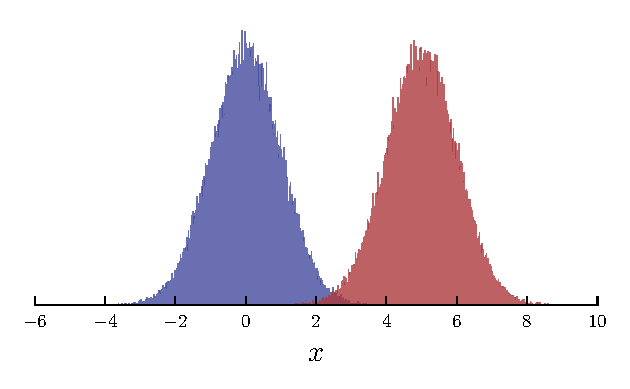
\includegraphics[width=.8\textwidth]{hist_normal.pdf}\\[-.8em]
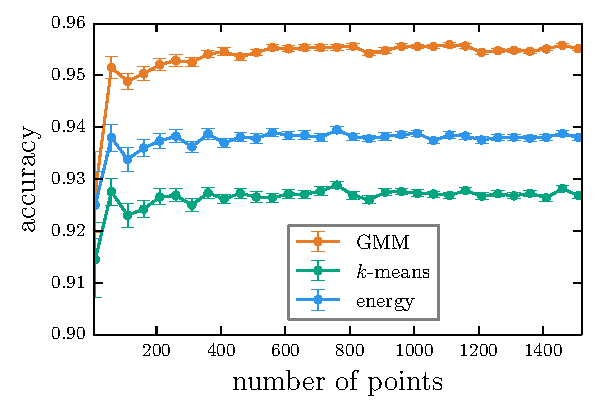
\includegraphics[width=\textwidth]{gauss1d.pdf}\\[-1em]
(a)
\end{minipage}
\begin{minipage}{0.49\textwidth}
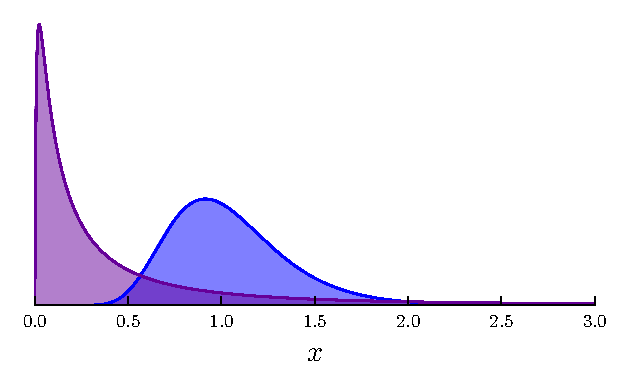
\includegraphics[width=.8\textwidth]{hist_lognormal.pdf}\\[-.8em]
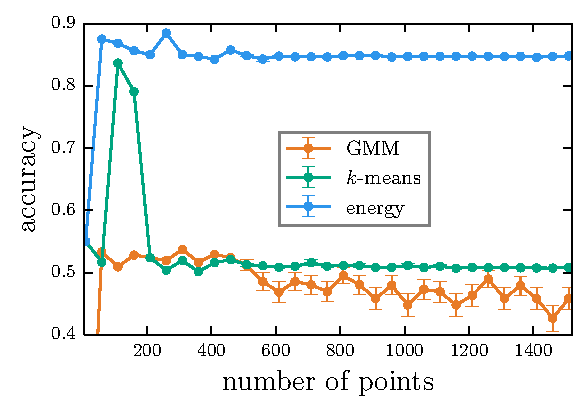
\includegraphics[width=\textwidth]{loggauss1d.pdf}\\[-1em]
(b)
\end{minipage}
\caption{
\label{fig:1d}
Energy statistics clustering by Algorithm~\ref{algo1d}
compared to $k$-means and GMM/EM.
We have the same number of points in both clusters, and for each case
we sample $100$ times from the distributions shown in the histograms. We 
plot the average value of 
\eqref{eq:accuracy} versus the total number of points 
(error bars are standard error). The dashed line indicates the
best possible classification accuracy computed from Bayes error.
(a) Data coming from \eqref{eq:two_normal}, where the
optimal accuracy is $\approx 0.956$.
(b) Data from \eqref{eq:two_lognormal}, where the optimal
accuracy is $\approx 0.852$.
}
\end{figure}

Let us consider two simple experiments with equal number of points
in each cluster. We plot the accuracy \eqref{eq:accuracy} versus the number
of points in each cluster.
The data is clustered using 
Algorithm~\ref{algo1d}, GMM through EM algorithm, and standard $k$-means 
algorithm. In the last two cases 
we use the initialization from $k$-means++ \cite{Vassilvitskii} 
and we run the algorithms
few times choosing the result with  best objective function value. 
Notice that Algorithm~\ref{algo1d} requires no initialization so we only
run it once.
Moreover, for each case we sample $100$ times
and show the average accuracy with error bars indicating
the standard error.
In  Fig.~\ref{fig:1d}a 
we have data sampled from two normal distributions with equal number of
points in each cluster,
\begin{equation}
\label{eq:two_normal}
x \sim \mathcal{N}\big(\mu_i,\sigma_i^2\big) 
\quad 
\mbox{with $\mu_1 = 0$, $\sigma_1=1$ and
$\mu_2 = 5$, $\sigma_2 = 2$.}
\end{equation}
For these distributions the optimal accuracy 
obtained from Bayes classification error
is $ \approx 0.956$ which is indicated by the dashed line in the plot.
We see that the three methods
perform closely. As expected, GMM has a slight advantage over the other
methods since
it corresponds to the true model of the data. 
Energy statistics performs slightly better
than $k$-means. On the other hand, in Fig.~\ref{fig:1d}b
we consider two clusters with lognormal distributions,
\begin{equation}
\label{eq:two_lognormal}
\log x \sim \mathcal{N}\big( \mu_i,\sigma_i^2\big) \quad
\mbox{with
$\mu_1 = 0$,
$\sigma_1 = 0.3$ and
$\mu_2 = -1.5$,
$\sigma_2 = 1.5$.}
\end{equation}
The optimal classification accuracy from Bayes error is $\approx 0.852$.
In this case,
Algorithm~\ref{algo1d} provides a very accurate clustering while
GMM and $k$-means basically cluster at chance.
Sometimes GMM/EM  was unable to estimate the parameters 
thus giving zero accuracy.
The two simple experiments of Fig.~\ref{fig:1d} illustrate
how energy statistics clustering is nonparametric, being able
to provide high quality clustering in settings where data comes
from very different distributions.


%%%%%%%%%%%%%%%%%%%%%%%%%%%%%%%%%%%%%%%%%%%%%%%%%%%%%%%%%%%%%%%%%%%%%%%%%%%%%%%
\section{Iterative Algorithms for Energy Statistics Clustering}
\label{sec:algo}

In this section we introduce an iterative algorithm to find a local
maximizer of \eqref{eq:qcqp2}. However, due to 
Proposition~\ref{th:kernel_kmeans} we can also find an approximate
solution by the well-known kernel $k$-means algorithm 
(see \cite{Dhillon2,Dhillon}), which 
for convenience will also be restated in the present context.

Consider the optimization problem 
written in the form \eqref{eq:max_prob} as follows:
\begin{equation}
\label{eq:maxQ}
\max_{\{ \C_1,\dotsc,\C_k \}} 
\bigg\{ Q = \sum_{j=1}^k \dfrac{Q_j}{n_j}  \bigg\},
\qquad Q_j = \sum_{x,y\in\C_j} \kk(x,y),
\end{equation}
where $Q_j$ represents an internal energy cost of cluster $\C_j$, and
$Q$ is the total energy cost where each $Q_j$ 
is weighted by the inverse
of the number of its elements. For a data point $x_i$ we denote
its own energy cost
with the entire cluster $\C_\ell$ by
\begin{equation}
\label{eq:costxij}
Q_\ell(x_i) \equiv \sum_{y\in\C_\ell} \kk(x_i, y) = 
G_{i \bullet} \cdot Z_{\bullet \ell},
\end{equation}
where we recall that $G_{i\bullet}$ ($G_{\bullet i}$) denotes
the $i$th row (column) of matrix $G$.

\subsection*{Kernel $\bm{k}$-Means Algorithm}

To optimize the kernel $k$-means objective function
\eqref{eq:J} we remove the global term and define the function
\begin{equation}
\label{eq:Jell}
J^{(\ell)}(x_i) \equiv 
\dfrac{1}{n_\ell^2} Q_\ell
-\dfrac{2}{n_\ell} Q_\ell(x_i) 
\end{equation}
which represents a cost depending on point $x_i$ and cluster $\C_\ell$. One
thus assigns  $x_i$ to cluster $\C_{j^\star}$ according
to $j^\star = \argmin_\ell J^{(\ell)}(x_i)$, for $\ell = 1,\dotsc,k$.
This procedure is performed for every data point and repeated until
convergence, i.e. until no new assignments are made.
The entire procedure is described in Algorithm~\ref{kmeans_algo}.
It can be shown that this algorithm converges provided $G$ is positive
semidefinite.

Notice that to compute the first term in \eqref{eq:Jell} requires
$\OO(n_\ell)$ operations, and although the second term requires
$\OO(n_\ell^2)$ it only needs to be computed once outside loop through
data points (step 1).
Therefore, the time complexity Algorithm~\ref{kmeans_algo} is
$\OO(n k \max_\ell n_\ell) = \OO(k n^2)$. For a sparse
Gram matrix $G$ having
$n'$ nonzero elements this complexity can be further reduced
to $\OO(k n')$. 

\begin{figure}
\begin{algorithm}[H]
\vspace{.5em}
\begin{algorithmic}[1]
    \INPUT number of clusters $k$, Gram matrix $G$, initial label
    matrix $Z = Z_0$
    \OUTPUT label matrix $Z$ 
  \STATE $q \leftarrow (Q_1, \dotsc, Q_k)^\top$ 
            have the costs of each cluster, according to \eqref{eq:maxQ}
  \STATE $n \leftarrow (n_1,\dotsc,n_k)^\top$ 
        have the number of points in each cluster, obtained 
        from $D = Z^\top Z$
  \REPEAT
    \FOR{ $i=1,\dotsc,n$}
        \STATE let $j$ be such that $x_i \in \C_j$
        \STATE $j^\star \leftarrow \argmin_{\ell} J^{(\ell)}(x_i)$
            according to \eqref{eq:Jell}, for $\ell=1,2,\dots,k$
        \IF{ $j^\star \ne j$} 
            \STATE move $x_i$ to $\C_{j^\star}$: $Z_{ij} \leftarrow 0$ and
            $Z_{ij^\star} \leftarrow 1$
            \STATE update $n$: $n_j \leftarrow n_j - 1$ and
                    $n_{j^\star} \leftarrow n_{j^\star} + 1$
            \STATE update $q$: $q_j \leftarrow q_j - 2Q_j(x_i)$ and
    $q_{j^\star} \leftarrow q_{j^\star} + 2Q_{j^\star}(x_i)$
    %    \ELSE
    %        \STATE Do nothing;
        \ENDIF
    \ENDFOR
  \UNTIL{convergence}
\end{algorithmic}
\caption{\label{kmeans_algo}
Kernel $k$-means algorithm 
to find a local solution to \eqref{eq:qcqp2}.
\hspace{\fill}
}
\end{algorithm}
\end{figure}

\subsection*{Hartigan's Method for Energy Statistics Clustering}

We now consider an algorithm based on Hartigan's method \cite{Hartigan} 
applied to \eqref{eq:maxQ}. This gives a local solution to 
\eqref{eq:qcqp2}. 
%This approach was also proposed in \cite{Kgroups}.
The method is based on the change
in the within energy statistic when moving a given data point to
another cluster.
Suppose point $x_i \in \mathcal{X}$
is currently assigned to  cluster $\C_j$, yielding
a total energy cost function \eqref{eq:maxQ} denoted by $Q^{(j)}$.
Let us consider the change in the total within energy by moving
$x_i$ to $\C_\ell$. 
Denote this new energy cost by $Q^{(\ell)}$.
A straightforward computation gives
\begin{equation}
\label{eq:changeQ}
\begin{split}
\Delta Q^{j \to \ell}(x_i) &\equiv Q^{(\ell)} - Q^{(j)} \\ 
&= 
\dfrac{1}{n_j - 1}\left[ \dfrac{Q_j}{n_j} - 2 Q_j(x_i) \right]
- \dfrac{1}{n_\ell + 1}\left[ \dfrac{Q_\ell}{n_\ell} - 2 \big(Q_\ell(x_i) + 
\kk(x_i,x_i)\big) 
\right].
\end{split}
\end{equation}
Thus, if $\Delta Q^{j\to \ell}(x_i) > 0$ we get closer to a 
maximum of \eqref{eq:maxQ} by
moving $x_i$ to $\C_\ell$, otherwise we keep $x_i$ in $\C_j$. Based on
this the algorithm goes as follows.
We start with an initial configuration for the label matrix $Z$, 
then for each
point $x_i$ 
we compute the cost of moving it to another cluster $\C_\ell$,
$\Delta Q^{j\to \ell}(x_i)$ for 
$\ell=1,\dots,k$ with $\ell \ne j$. Hence, let us choose
$j^\star = \argmax_\ell \Delta^{j \to \ell}(x_i)$.
If $\Delta Q^{j \to j^\star}(x_i) > 0$ 
we move $x_i$ to cluster $\C_{j^\star}$, otherwise 
we keep $x_i$ in its original cluster $\C_j$. We update $Z$ accordingly.
The process is repeated
until no points are assigned to new clusters. 
This whole procedure is described in Algorithm~\ref{algo}.
Note that this ensures that the objective function is
monotonically increasing at each iteration and consequently the algorithm
converges in a finite number of steps.

\begin{figure}
\begin{algorithm}[H]
\vspace{.5em}
\begin{algorithmic}[1]
    \INPUT number of clusters $k$, Gram matrix $G$, 
                initial label matrix $Z=Z_0$
    \OUTPUT label matrix $Z$
  \STATE $q \leftarrow (Q_1, \dotsc, Q_k)^\top$ 
            have the energy costs of each cluster, according to \eqref{eq:maxQ}
  \STATE $n \leftarrow (n_1,\dotsc,n_k)^\top$ have the number of points 
        in each cluster, obtained from $D=Z^\top Z$
  \REPEAT
    \FOR{ $i=1,\dotsc,n$}
        \STATE let $j$ be such that $x_i \in \C_j$
        \STATE $j^\star \leftarrow \argmax_{\ell} \Delta Q^{j\to \ell}(x_i)$, 
            for $\ell=1,2,\dots,k$ and $\ell \ne j$ \label{stepmove}
        \IF{ $\Delta Q^{j \to j^\star}(x_i) > 0$ }
            \STATE move $x_i$ to $\C_{j^\star}$: $Z_{ij} \leftarrow 0$ and 
            $Z_{ij^\star} \leftarrow 1$
            \STATE update $n$: $n_j \leftarrow n_j - 1$ and
                    $n_{j^\star} \leftarrow n_{j^\star} + 1$
            \STATE update $q$: $q_j \leftarrow q_j - 2Q_j(x_i)$ and
    $q_{j^\star} \leftarrow q_{j^\star} + 2\left(Q_{j^\star}(x_i)+
    G_{ii}\right)$
    %    \ELSE
    %        \STATE Do nothing;
        \ENDIF
    \ENDFOR
  \UNTIL{convergence}
\end{algorithmic}
\caption{\label{algo}
Hartigan's method to find a local solution to \eqref{eq:qcqp2}.
\hspace{\fill}
}
\end{algorithm}
\end{figure}

Computing $G$ requires $\OO( D n^2)$ operations, where 
$D$ is the dimension of each data point and $n$ is the data size. However,
both Algorithms~\ref{kmeans_algo} and \ref{algo} 
assume that $G$ is given. There are more efficient
methods to compute $G$, specially if it is sparse, but we will not consider
this further and just assume that $G$ is given.
The computation of each cluster cost
$Q_j$ has complexity $\OO(n_j^2)$, and overall to compute $q$
we have $\OO(n_1^2+\dots + n_k^2) = \OO(k \max_j n_j^2)$. 
These operations only need to be performed a single time. For
each point $x_i$ we need to compute $Q_j(x_i)$ once, which is
$\OO(n_j)$, and we need to compute $Q_\ell(x_i)$ for each $\ell\ne j$. 
The cost of computing 
\eqref{eq:costxij} is $\OO(n_j)$, thus the cost of step~$8$ in
Algorithm~\ref{algo} is $\OO(k \max_j n_j)$ for $j=1,\dotsc,k$.
For the 
entire dataset this gives a time complexity
of $\OO(n k  \max_j n_j) =\OO(k n^2)$. This is the same cost as
in kernel $k$-means, Algorithm~\ref{kmeans_algo}. Again, if $G$ is sparse
this can be reduced to $\OO(k n')$ where $n'$ is the number of nonzero
entries of $G$.

Let us mention some important results about Hartigan's method.

\begin{theorem}[Telgarsky-Vattani \cite{Telgarsky}]
Hartigan's method has the cost function strictly decreasing in each
iteration. Moreover, if $n > k$ then 
\begin{enumerate}
\item \label{noempty} the resulting partition has no empty clusters, and
\item \label{diffmean} the resulting partition has distinct means.
\end{enumerate}
\end{theorem}

Both conditions of the  above theorem are not satisfied 
by Lloyd's method, and consequently by (kernel) $k$-means algorithm.
The next result indicates that Hartigan's can potentially 
escape local optima of Lloyd's method.

\begin{theorem}[Telgarsky-Vattani \cite{Telgarsky}]
The set of local optima of Hartigan's method is a (possibly strict) subset
of local optima of Lloyd's method.
\end{theorem}

This means that Algorithm~\ref{kmeans_algo} cannot
improve on a local optima of Algorithm~\ref{algo}. On the other hand,
Algorithm~\ref{algo} might improve on a local optima of 
Algorithm~\ref{kmeans_algo}. Lloyd's method forms Voronoi partitions,
while Hartigan's method groups data
in regions formed by the intersection of spheres called circlonoi cells.
It can be shown that the circlonoi cells are contained within
a smaller volume of a Voronoi cell, and this excess volume grows
exponentially with the dimension of $\mathcal{X}$ 
\cite[Theorems 2.4 and 3.1]{Telgarsky}. 
Points in this excess volume
force Hartigan's method to iterate, contrary
to Lloyd's method. Therefore, Hartigan's method 
can escape local
optima of Lloyd's method. 
Moreover, this improvement should be more prominent as
dimension increases. Also, the improvement grows as $k$
increases.
The empirical results of \cite{Telgarsky} show that 
an implementation of Hartigan's method has comparable execution time 
as an implementation of
Lloyd's method,
but no explicit complexity was provided. In our case, we showed that both
Algorithms~\ref{kmeans_algo} and \ref{algo} have the same time complexity.

In \cite{Slonin} Hartigan's method was applied to $k$-means problem
with any Bregman divergence. They showed that the number of Hartigan's
local minima is upper bounded by $\mathcal{O}(1/k)$ 
\cite[Proposition 5.1]{Slonin}. 
In addition, they provide examples where
\emph{any} initial partition correspond to a local optima of Lloyd's 
method, while  the number of local optima in Hartigan's method is small and 
correspond to true partitions of the data. Empirically, the number of
Hartigan's local optima was considerably smaller than the number of Lloyd's
local optima.
These results indicate that Hartigan's method
provides several advantages over Lloyd's method. 
We will see this explicitly in the following 
numerical results where Algorithm~\ref{algo}
outperforms Algorithm~\ref{kmeans_algo} when using the same kernel.


%%%%%%%%%%%%%%%%%%%%%%%%%%%%%%%%%%%%%%%%%%%%%%%%%%%%%%%%%%%%%%%%%%%%%%%%%%%%%%%
\section{Numerical Experiments}
\label{sec:numerics}

In the experiments below we fix the semimetric 
according to the traditional energy distance \eqref{eq:energy}, and
the point $x_0=0$ is chosen in the corresponding kernel  
\eqref{eq:kernel_semimetric}. Therefore,
\begin{equation}
\label{eq:standard_metric}
\rho(x,y) = \| x-y\| \qquad \mbox{and} \qquad \kk(x,y) = 
\tfrac{1}{2}\left( \| x \| + \| y \| - \| x-y \| \right).
\end{equation}
We will consider other kernels as well 
but \eqref{eq:standard_metric} will be the
standard kernel for energy statistics and will always be present in the
experiments as a reference.

Let us briefly mention that we compared Algorithm~\ref{algo} and
Algorithm~\ref{algo1d} for several univariate distributions and
both perform almost indistinguishable regarding the clustering quality.
However, we omit these results since we will analyse more interesting 
scenarios in high dimensions and $k > 2$ number of clusters.

The main goal of the 
experiments  to follow
is to compare Algorithm~\ref{algo} based on Hartigan's method to
kernel $k$-means, as described in Algorithm~\ref{kmeans_algo}, which
is based on Lloyd's method. 
From the discussion in the end of the previous section we can anticipate
that Algorithm~\ref{algo} will be superior than Algorithm~\ref{kmeans_algo}.
Another goal is to illustrate the nonparametric aspect of energy statistics.
To this end we also compare
Algorithm~\ref{algo} to standard $k$-means and GMM/EM since 
these are the most used
clustering algorithms in practice.
Moreover, for every algorithm, we always
choose the initialization procedure from $k$-means++%
\footnote{Notice that we just use the initialization
procedure and not the full $k$-means++ algorithm.} \cite{Vassilvitskii}.
Our measure of clustering quality will be the accuracy \eqref{eq:accuracy}
based on the ground truth. Furthermore, in every experiment, we sample
data many times and show the average value of the accuracy with error bars
indicating the standard error. Whenever possible, 
we also indicate the optimal 
accuracy computed from
Bayes classification error.

From the results of \cite{Telgarsky}, the improvement of Hartigan's 
over Lloyd's method should be more accentuated in high dimensions.
Thus, let us analyse
how the algorithms degrade as the number of dimensions increase, while
keeping the number of points in each cluster fixed. Consider
two clusters with multivariate normal distributions given by
\begin{equation}
\label{eq:gauss1}
\begin{split}
x &\in \C_i  \sim 
\mathcal{N}(\mu_i,\Sigma_i) \qquad (i=1,2),  \\
\mu_1 &= (\underbrace{0,\dotsc,0}_{\times D})^\top , \quad
\mu_2 = 0.7 \times (\underbrace{1,\dots,1}_{\times 10},
\underbrace{0,\dots,0}_{\times (D-10)})^\top, \quad
\Sigma_1 = \Sigma_2 = I_D.
\end{split}
\end{equation}
Note that the Bayes error
is fixed as $D$ increases, giving an optimal 
accuracy of $\approx 0.86$.
For each $D$ we sample $100$ times, picking $100$ points for each cluster.
We apply each algorithm to the resulting dataset 
and compute the average of the accuracy \eqref{eq:accuracy} (error bars
are standard error).
Algorithm~\ref{algo} and Algorithm~\ref{kmeans_algo} 
both use the standard
kernel \eqref{eq:standard_metric}.
The results are shown in Fig.~\ref{fig:gauss}a.
Note that GMM/EM is unable to estimate the covariance matrices
when the number of dimensions exceeds the number of points in each cluster,
giving zero accuracy when dimensions are $\gtrsim 100$.
We see that Algorithm~\ref{algo} performs better than all the other ones,
and in particular it outperforms kernel $k$-means algorithm as the number
of dimensions increase. Note also that although GMM and $k$-means are
parametric they are consistent models to the data.

\begin{figure}
\begin{minipage}{0.49\textwidth}
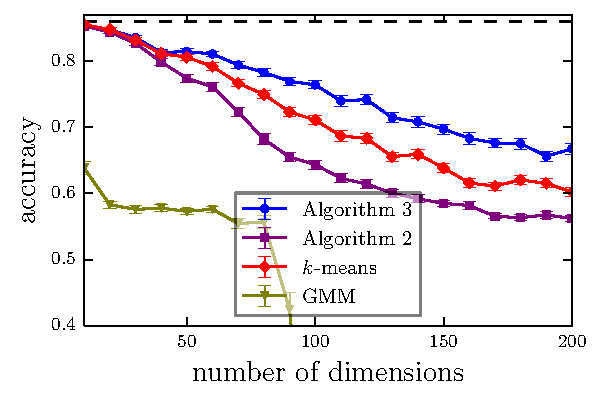
\includegraphics[width=1\textwidth]{gauss_dim.pdf}\\[-1.0em] (a)
\end{minipage}
\begin{minipage}{0.49\textwidth}
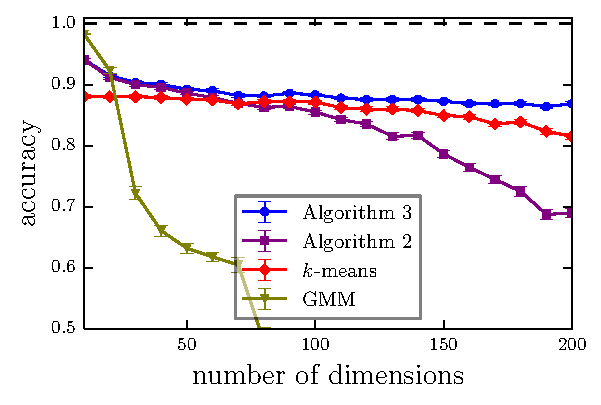
\includegraphics[width=1\textwidth]{gauss_cov_squareroot.pdf}\\[-1.0em] (b)
\end{minipage}
\begin{minipage}{0.49\textwidth}
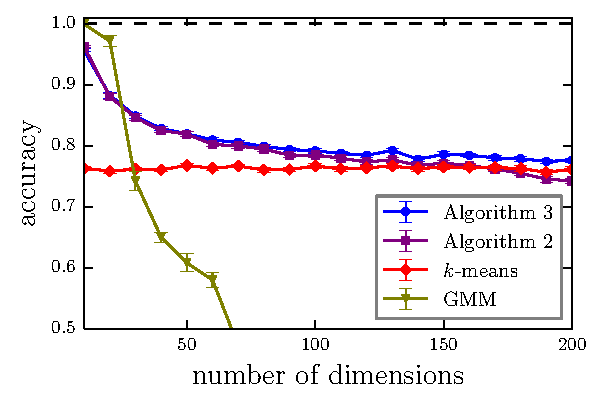
\includegraphics[width=1\textwidth]{gauss_cov_linear.pdf}\\[-1.0em] (c)
\end{minipage}
\begin{minipage}{0.49\textwidth}
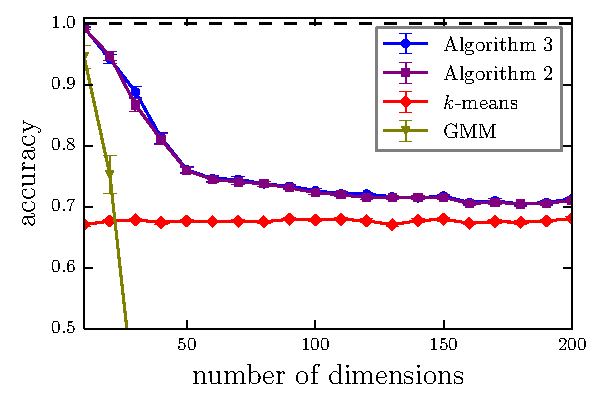
\includegraphics[width=1\textwidth]{gauss_cov_square.pdf}\\[-1.0em] (d)
\end{minipage}
\caption{
\label{fig:gauss}
Comparison of Algorithm~\ref{algo}, Algorithm~\ref{kmeans_algo},
standard $k$-means and GMM/EM as the number of dimensions increase
in gaussian settings.
We compute the average of \eqref{eq:accuracy} over $100$ samples with
error bars being standard error. We have two clusters with $100$ points
each. 
(a) Data as in \eqref{eq:gauss1}, where the optimal accuracy
from Bayes error is the dashed line equal to $\approx 0.86$.
(b) Data from \eqref{eq:gauss2} with $q=1/2$ in \eqref{eq:cov}. 
(c) Data from \eqref{eq:gauss2} with $q=1$ in \eqref{eq:cov}.
(d) Data from \eqref{eq:gauss2} with $q=2$ in \eqref{eq:cov}.
The optimal accuracy from Bayes error in (b--d) is $\approx 1$.
}
\end{figure}

Let us now consider the same experiment as before with data distributed as
\begin{equation}
\label{eq:gauss2}
x \in \C_i  \sim 
\mathcal{N}(\mu_i,\Sigma_i) \quad (i=1,2),  \quad
\mu_1 = (\underbrace{0,\dotsc,0}_{\times D})^\top , \quad
\mu_2 = (\underbrace{1,\dots,1}_{\times 10},
\underbrace{0,\dots,0}_{\times (D-10)})^\top, 
\end{equation}
where
\begin{equation}
\label{eq:cov}
(\Sigma_1)_{ij} = \begin{cases}
i^{-q} \delta_{ij} & \mbox{if $i \le 10$} \\
\delta_{ij} & \mbox{if $10 < i \le D$}
\end{cases} \qquad
(\Sigma_2)_{ij} = \begin{cases}
i^{\,q} \delta_{ij} & \mbox{if $i \le 10$} \\
\delta_{ij} & \mbox{if $10 < i \le D$}
\end{cases} 
\end{equation}
and we choose $q \in \{ 1/2, 1, 2\}$. In these cases,
the best possible accuracy from Bayes classification error is $\approx 1$.
In Fig.~\ref{fig:gauss}b--d we have $q=1/2$, $q=1$, and $q=2$, respectivelly.
Again, GMM/EM is unable to estimate the covariance matrices
as dimensions get larger than $\gtrsim 100$, and it gives poor results even
for number of dimensions much lower than this. Note that GMM requires
a larger number of points to estimate the parameters accurately.
Algorithm~\ref{algo} outperforms
Algorithm~\ref{kmeans_algo}, and $k$-means degrades faster as 
$q$ increases.

To summarize, in the experiments of Fig.~\ref{fig:gauss}
we see a better performance of Algorithm~\ref{algo} compared
to the other ones, and in particular to kernel $k$-means,
where we recall that both find local solutions
to the same optimization problem \eqref{eq:qcqp2}.
Algorithm~\ref{algo} is more robust as the number of dimensions
increase.

Let us now
consider the effect of having 
unbalanced clusters. We generate data as
\begin{equation}
\label{eq:gauss3}
\begin{split}
x &\in \C_i \sim  
\dfrac{n_i}{N} \mathcal{N}(\mu_i,\Sigma_i) \quad (i=1,2), \quad 
\mu_1 = (0,0,0,0)^\top , \quad
\mu_2 = 1.5\times (1,1,0,0)^\top, \\
\Sigma_1 &= I_4, \quad
\Sigma_2 = \left( 
\begin{smallmatrix} 
1/2 & 0 & 0 & 0\\
0 & 1/2 & 0 & 0 \\
0 & 0 & 1 & 0 \\
0 & 0 & 0 & 1 
\end{smallmatrix}\right), \quad
n_1 = N - m, \quad  n_2 = N + m, \quad N=200.
\end{split}
\end{equation}
We then increase $m$, 
that is we make the clusters progressively more unbalanced,
and plot the average of \eqref{eq:accuracy} 
over
$100$ samples for each $m$
(error bars are standard error). The results are in Fig.~\ref{fig:unbalanced}.
As expected, GMM
works better than the other algorithms since it is a fuzzy clustering.
The other methods based on hard assignments degrade similarly
and  more rapidly than GMM. This indicates that a fuzzy version of
Algorithm~\ref{algo} should compensate for this effect.

\begin{figure}
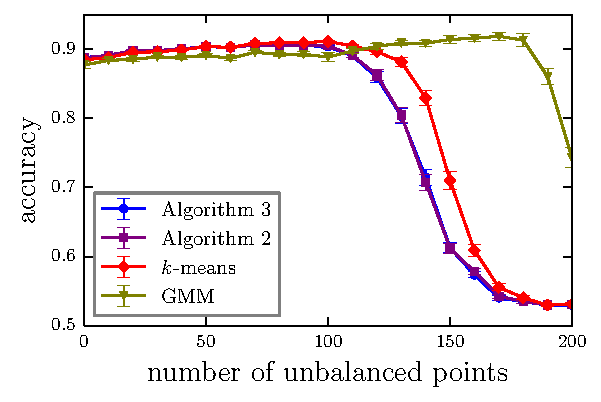
\includegraphics[width=0.5\textwidth]{gauss_pi.pdf}\vspace{-1em}
\caption{
\label{fig:unbalanced}
Comparison of Algorithm~\ref{algo}, Algorithm~\ref{kmeans_algo}, 
$k$-means, and GMM/EM. The data is distributed as \eqref{eq:gauss3} where
we make the clusters progressively more unbalanced.
}
\end{figure}

Besides the standard kernel from energy statistics 
\eqref{eq:standard_metric}, 
let us consider two other semimetrics with their respective generating
kernels,
\begin{align}
\rho_{1/2}(x,y) &= \| x-y \|^{1/2} & 
 \kk_{1/2}(x,y) &= \tfrac{1}{2} \left( 
\| x \|^{1/2} + \| y \|^{1/2} 
- \| x-y \|^{1/2} \right), \label{eq:rhohalf}\\
\rho_{e}(x,y) &= 
2 - 2 e^{-\tfrac{1}{2}\| x- y\|} &
 \kk_{e}(x,y) &= e^{-\tfrac{1}{2}\| x-y\|}.
\label{eq:rhoe}
\end{align}
The kernel \eqref{eq:rhohalf} corresponds to the energy distance
\eqref{eq:energy2} with $\alpha=1/2$.
Now consider data normally distributed in $D=20$ as
\begin{equation}
\label{eq:20gauss}
\begin{split}
x &\in \C_i \sim \mathcal{N}(\mu_i,\Sigma_i) \qquad (i=1,2), \\
\mu_1 &= (\underbrace{0,\dotsc,0}_{\times 20})^\top ,\quad
\mu_2 = \tfrac{1}{2} 
(\underbrace{1,\dotsc,1}_{5},\underbrace{0,\dotsc,0}_{15})^\top, \quad
\Sigma_1 = \tfrac{1}{2} I_{20},  \quad
\Sigma_2 = I_{20}.
\end{split}
\end{equation}
We sample an equal number of points for each cluster, which is progressively
increased. The optimal accuracy based on Bayes
classification error is $\approx 0.90$. 
Clustering results are shown in Fig.~\ref{fig:consist}a.
Algorithm~\ref{algo} outperforms the other ones, and in 
particular the kernel \eqref{eq:rhoe} provides better results.
As the number of points get large enough GMM starts to approach
optimal Bayes, as it should since it is a
consistent model to the data. However, 
Algorithm~\ref{algo} with kernel \eqref{eq:rhoe} approach optimal Bayes
with a much smaller number of points. Moreover, Algorithm~\ref{algo} 
outperforms
Algorithm~\ref{kmeans_algo} for any of the kernel choices.
%Standard $k$-means performs poorly in this example.

Now consider the same parameters as in \eqref{eq:20gauss} but with
lognormal distributions, 
\begin{equation}
\label{eq:20loggauss}
\log x \in \C_i \sim \mathcal{N}(\mu_i, \Sigma_i) \qquad (i=1,2).
\end{equation}
The same previous experiment is shown in 
Fig.~\ref{fig:consist}b.
Note that Algorithm~\ref{algo} still performs accurately, 
while $k$-means works almost at chance,
and GMM is not even able to estimate the parameters. Again, the
kernel \eqref{eq:rhoe}
provides better results than \eqref{eq:standard_metric} or
\eqref{eq:rhohalf}. 
The experiments in Fig.~\ref{fig:consist}
illustrate how energy statistics clustering is nonparametric.

\begin{figure}
\begin{minipage}{0.49\textwidth}
\centering
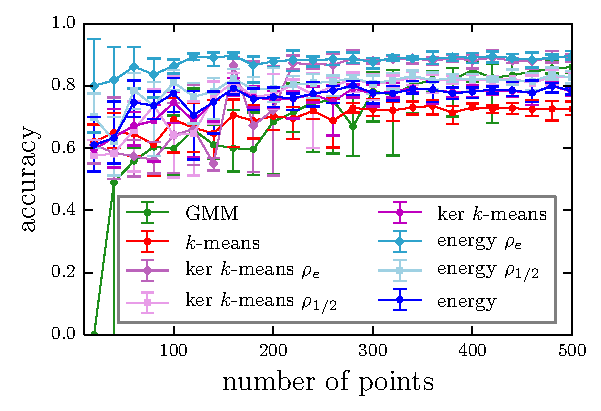
\includegraphics[width=1\textwidth]{gauss.pdf}\\[-1.0em]
(a)
\end{minipage}
\begin{minipage}{0.49\textwidth}
\centering
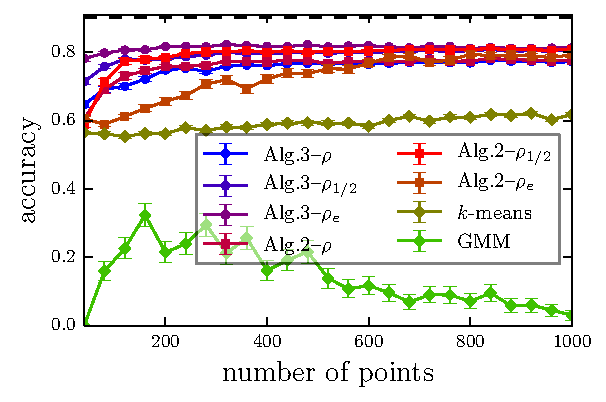
\includegraphics[width=1\textwidth]{loggauss.pdf}\\[-1.0em]
(b)
\end{minipage}
\caption{
\label{fig:consist}
Algorithm~\ref{algo} and Algorithm~\ref{kmeans_algo} with kernels
\eqref{eq:standard_metric}, \eqref{eq:rhohalf} and \eqref{eq:rhoe}, 
$k$-means, and GMM. The optimal accuracy in both cases
is $\approx 0.9$. We show the average of \eqref{eq:accuracy}
over $100$ samples with standard error.
(a) Data distributed as in 
\eqref{eq:20gauss}. 
(b) Data distributed as in \eqref{eq:20loggauss}.
}
\end{figure}


\begin{figure}
\begin{minipage}{0.24\textwidth}
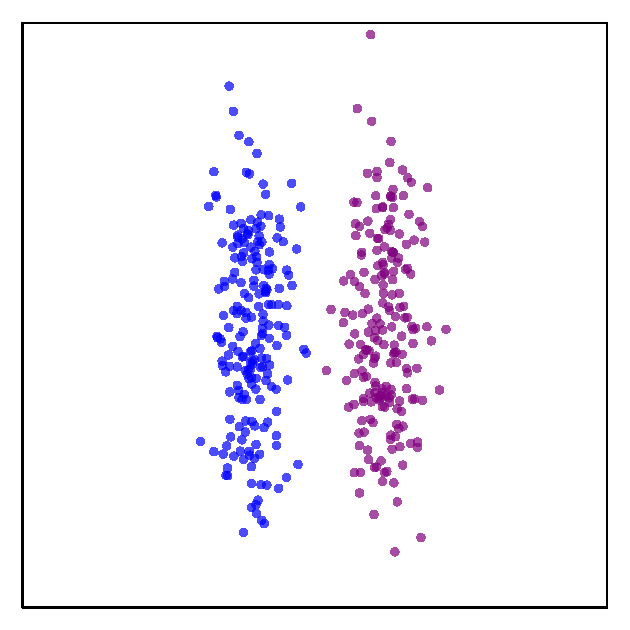
\includegraphics[width=1\textwidth]{2cigars.pdf}\\[-1em] (a)
\end{minipage}
\begin{minipage}{0.24\textwidth}
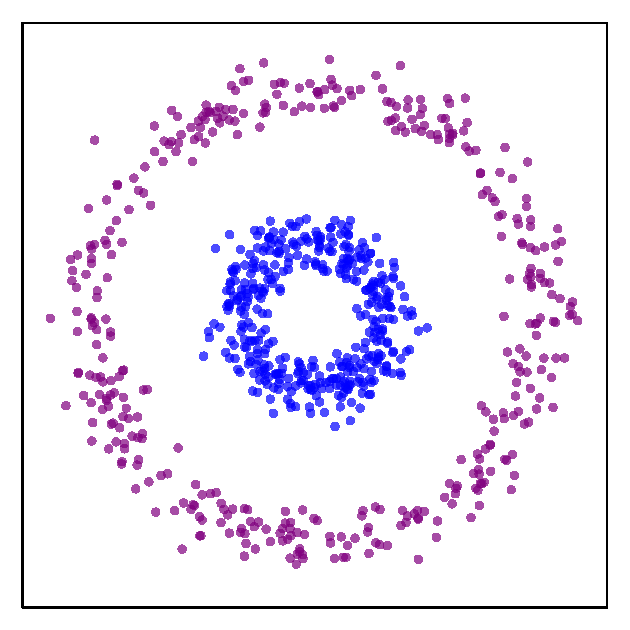
\includegraphics[width=1\textwidth]{2circles.pdf}\\[-1em] (b)
\end{minipage}
\begin{minipage}{0.24\textwidth}
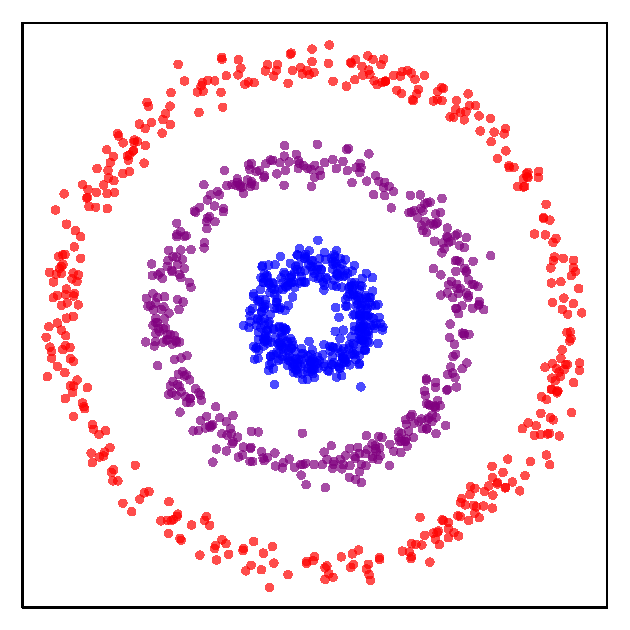
\includegraphics[width=1\textwidth]{3circles.pdf}\\[-1em] (c)  
\end{minipage}
\begin{minipage}{0.23\textwidth}
\vspace{-0.9em}
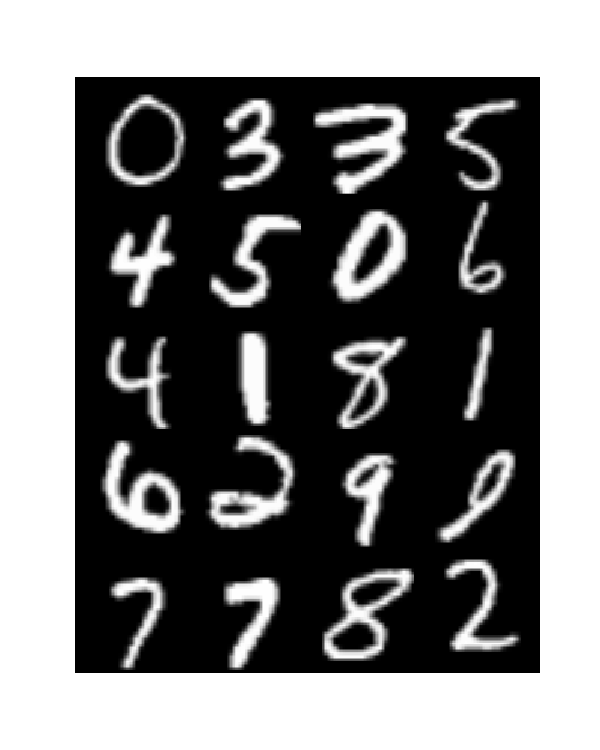
\includegraphics[width=1\textwidth]{mnist.pdf}\\[-1.8em] (d)  
\end{minipage}
\caption{\label{fig:other}
(a) Parallel cigars. (b) Two  
concentric circles with noise. (c) Three
concentric circles with noise. (d) MNIST handwritten digits.
Clustering results are in Table~\ref{table:other}
and Table~\ref{table:mnist}.
}
\end{figure}

Consider the following choices of semimetric and 
corresponding generating kernel:
\begin{align}
\rho_{\alpha}(x,y) &= \| x - y\|^\alpha & 
\kk_{\alpha}(x,y) &= \tfrac{1}{2}\left(
\| x \|^\alpha +
\| y \|^\alpha -
\| x-y \|^\alpha \right) ,
\label{eq:rhoalpha} \\
%
\widetilde{\rho}_{\sigma}(x,y) &= 2 - 2 e^{-\tfrac{\|x-y\|}{2 \sigma}} &
\widetilde{\kk}_{\sigma}(x,y) &= e^{-\tfrac{\|x-y\|}{2\sigma}} ,
\label{eq:rhoesigma} \\
%
\widehat{\rho}_{\sigma}(x,y) &= 2 - 2 e^{-\tfrac{\|x-y\|^2}{2 \sigma^2}} &
\widehat{\kk}_{\sigma}(x,y) &= e^{-\tfrac{\|x-y\|^2}{2\sigma^2}} .
\label{eq:rhogsigma} 
\end{align}
In Fig.~\ref{fig:other} we have examples of
complex two dimensional datasets. The two parallel cigars of 
Fig.~\ref{fig:other}a have $200$ points each. For the concentric circles
of Fig.~\ref{fig:other}b and Fig.~\ref{fig:other}c we
sample $400$ points for each class.
We apply Algorithm~\ref{algo} and Algorithm~\ref{kmeans_algo}, besides
$k$-means and GMM, using the above kernels 
\eqref{eq:rhoalpha}--\eqref{eq:rhogsigma}. The results are shown
in Table~\ref{table:other} where the respective choice of parameters for the
kernels are indicated. For the data in Fig.~\ref{fig:other}a 
the semimetrics $\rho_1$ and $\rho_{1/2}$ are
able to provide more accurate results compared to $k$-means. However,
the gaussian kernel $\widetilde{\rho}_2$ gives very accurate
results, similar to GMM,
which is the true model of the data. For the data shown in
Fig.~\ref{fig:other}b we see
that the choice of kernel is very sensitive, and only \eqref{eq:rhoesigma}
was able to cluster accurately. The same kernel choice to the case
of Fig.~\ref{fig:other} still provides better results than
the others, but they are less accurate compared to Fig.~\ref{fig:other}b.


\newcolumntype{g}{>{\columncolor{gray!20}}l}
\begin{table}[h]
\renewcommand*{\arraystretch}{0.75}
\begin{tabular}{@{}r  l g  l g  l g@{}}
\toprule[1pt]
 & & \emph{Fig.~\ref{fig:other}a}
 & & \emph{Fig.~\ref{fig:other}b}
 & & \emph{Fig.~\ref{fig:other}c} \\
\midrule[0.5pt]
\multirow{4}{*}{\emph{Algorithm \ref{algo}}~~~~} 
& $\rho_{1}$ & $0.766\pm0.066$
& $\rho_{1}$ & $0.522\pm0.006$
& $\rho_{1}$ & $0.437\pm0.030$ \\
& $\rho_{1/2}$ & $0.859\pm0.062$
& $\rho_{1/2}$ & $0.524\pm0.007$
& $\rho_{1/2}$ & $0.547\pm0.026$ \\
& $\widetilde{\rho}_{2}$ & $0.971\pm0.015$
& $\widetilde{\rho}_{1}$ & $\bm{0.9999\pm0.0001}$
& $\widetilde{\rho}_{2}$ & $\bm{0.677\pm0.003}$ \\
& $\widehat{\rho}_{2}$  & $\bm{0.998\pm0.001}$
& $\widehat{\rho}_{1}$  & $0.597\pm0.052$
& $\widehat{\rho}_{2}$ & $0.645\pm0.012$ \\
\arrayrulecolor{gray!80}\midrule[0.5pt]
\multirow{4}{*}{\emph{Algorithm \ref{kmeans_algo}}~~~~} 
& $\rho_{1}$ & $0.758\pm 0.069$
& $\rho_{1}$ & $0.516\pm 0.002$
& $\rho_{1}$  & $0.452\pm 0.030$ \\
& $\rho_{1/2}$ & $0.901\pm 0.060$
& $\rho_{1/2}$ & $0.524\pm 0.007$
& $\rho_{1/2}$ & $0.570\pm 0.016$ \\
& $\widetilde{\rho}_{2}$ & $0.971\pm 0.015$
& $\widetilde{\rho}_{1}$ & $\bm{0.9999\pm 0.0001}$
& $\widetilde{\rho}_{2}$ & $\bm{0.673\pm 0.002}$ \\
& $\widehat{\rho}_{2}$ & $\bm{0.998\pm 0.001}$
& $\widehat{\rho}_{1}$ & $0.528\pm 0.008$
& $\widehat{\rho}_{2}$ & $0.640\pm 0.013$ \\
\arrayrulecolor{gray!80}\midrule[0.5pt]
\emph{$k$-means}~~~~ 
& & $0.599\pm0.046$
& & $0.521\pm0.005$
& & $0.360\pm0.004$ \\
\emph{GMM}~~~~
& & $0.9995\pm0.0003$
& & $0.598\pm0.018$
& & $0.479\pm0.021$ \\
\arrayrulecolor{black}\bottomrule[1pt]
\end{tabular}
\caption{\label{table:other}
Clustering the data shown in Fig.~\ref{fig:other} with Algorithm~\ref{algo}
and Algorithm~\ref{kmeans_algo}, besides $k$-means and GMM, with kernels 
\eqref{eq:rhoalpha}--\eqref{eq:rhogsigma}. 
We sample $10$ times and show the average
accuracy \eqref{eq:accuracy} with standard error.
}
\end{table}

Next we consider 
the well-known MNIST handwritten digit dataset 
as illustrated in Fig.~\ref{fig:other}d.
Each data point is an $8$-bit gray scale
image forming a $784$-dimensional vector 
corresponding to the digits $\{0,1,\dotsc,9 \}$.
Besides the kernel \eqref{eq:rhoalpha}, we
consider the gaussian kernel \eqref{eq:rhogsigma} with 
\begin{equation}
\label{eq:sigma}
\sigma^2 = \dfrac{1}{n^2} \sum_{i,j=1}^n \| x_i - x_j \|^2 ,
\end{equation}
which is computed from a sample  $\{ x_i \}_{i=1}^n$.
We consider subsets of the  classes $\{0,1,\dotsc,9 \}$, 
where we sample $100$ points 
for each class. We perform clustering through 
Algorithm~\ref{algo},
Algorithm~\ref{kmeans_algo}, and $k$-means.
The results are shown in Table~\ref{table:mnist} where the kernel
and its parameter for each case is indicated.
Algorithm~\ref{algo} performed slightly better than $k$-means, except
for the last column where all the methods are comparable. 
Unsupervised clustering on MNIST dataset without any feature extraction
or dimensionality reduction is not an easy task. For instance,
the same experiment was performed in \cite{Sapiro} where a low-rank
transformation is learned then subsequently used in subspace clustering,
providing very accurate results. One could explore analogous methods
for learning a better representation of the data and subsequently apply
Algorithm~\ref{algo} for clustering.

\newcolumntype{g}{>{\columncolor{gray!20}}l}
\begin{table}[h]
\renewcommand*{\arraystretch}{0.75}
\begin{tabular}{@{}rl|l|l|l|l@{}}
\toprule[1pt]
\emph{Class Subset}~~~~ & & $\{0,1,2\}$ &
$\{0,1,\dotsc,4\}$ &
$\{0,1,\dotsc,6\}$ &
$\{0,1,\dotsc,8\}$ \\
\midrule[0.5pt]
\multirow{3}{*}{\emph{Algorithm \ref{algo}}~~~~} 
& $\rho_{1}$\hspace{1em} 
&$0.907\pm 0.007$
&$0.866\pm 0.006$
&$0.715\pm 0.013$
&$0.616\pm 0.019$
\\
& $\rho_{1/2}$ 
&$\bm{0.918\pm 0.006}$
&$0.849\pm 0.025$
&$0.711\pm 0.010$
&$0.642\pm 0.009$
\\
& $\widetilde{\rho}_{\sigma}$ 
&$0.900\pm 0.007$
&$\bm{0.871\pm 0.005}$
&$\bm{0.719\pm 0.010}$
&$0.630\pm 0.016$
\\
\arrayrulecolor{gray!80}\midrule[0.5pt]
\multirow{3}{*}{\emph{Algorithm \ref{kmeans_algo}}~~~~} 
& $\rho_{1}$ 
&$0.914\pm 0.006$
&$0.845\pm 0.023$
&$0.664\pm 0.022$
&$0.614\pm 0.014$
\\
& $\rho_{1/2}$ 
&$0.895\pm 0.011$
&$0.822 \pm 0.026$
&$0.669\pm 0.021$
&$0.591\pm 0.019$
\\
& $\widetilde{\rho}_{\sigma}$ 
&$0.896\pm 0.007$
&$0.869\pm 0.006$
&$0.705\pm 0.016$
&$\bm{0.646\pm 0.020}$
\\
\arrayrulecolor{gray!80}\midrule[0.5pt]
\emph{$k$-means}~~~~ &
&$0.871\pm 0.015$
&$0.840\pm 0.022$
&$0.707\pm 0.012$
&$0.634\pm 0.011$
\\
\arrayrulecolor{black}\bottomrule[1pt]
\end{tabular}
\caption{\label{table:mnist}
Clustering the data shown in Fig.~\ref{fig:other}d with Algorithm~\ref{algo},
Algorithm~\ref{kmeans_algo}, and $k$-means.
We use the kernel \eqref{eq:rhoalpha} with $\alpha\in\{1,2\}$ and
the gaussian kernel 
\eqref{eq:rhogsigma} with $\sigma$ given by \eqref{eq:sigma}. 
For each subset of digits we sample $10$ times and show the average
accuracy \eqref{eq:accuracy} with standard error. We sample $100$ points for 
each class.
}
\end{table}


%Energy standard  : 0.991 0.00221108319357
%Energy half      : 0.993 0.000816496580928
%Energy rbf       : 0.99 0.00235702260396
%Kernel standard  : 0.9915 0.00183333333333
%Kernel half      : 0.992 0.00110554159679
%Kernel rbf       : 0.99 0.00235702260396
%k-means          : 0.9865 0.00258736244938
%
%
%%%%%%%%%%%%%%%%%%
%Energy standard  : 0.907333333333 0.00745024649522
%Energy half      : 0.918 0.00638671460587
%Energy rbf       : 0.899666666667 0.00708763485947
%Kernel standard  : 0.913666666667 0.00648740470089
%Kernel half      : 0.895333333333 0.0113442213494
%Kernel rbf       : 0.895666666667 0.00723588451341
%k-means          : 0.870666666667 0.0152412695107
%
%
%
%Energy standard  : 0.82975 0.0289550657629
%Energy half      : 0.857 0.0138232895265
%Energy rbf       : 0.85475 0.0164335784295
%Kernel standard  : 0.84875 0.016386181509
%Kernel half      : 0.79025 0.036198622595
%Kernel rbf       : 0.8545 0.0145334862377
%k-means          : 0.83425 0.01634289686
%
%
%%%%%%%%%%%%%%%%%%%%%
%Energy standard  : 0.8662 0.00636972003571
%Energy half      : 0.8494 0.0250138628231
%Energy rbf       : 0.8714 0.00536697721669
%Kernel standard  : 0.845 0.0234932614452
%Kernel half      : 0.8224 0.0261921107715
%Kernel rbf       : 0.8688 0.00640971484892
%k-means          : 0.8398 0.0224151734323
%
%
%Energy standard  : 0.703333333333 0.0166295883857
%Energy half      : 0.709833333333 0.0133690493859
%Energy rbf       : 0.702 0.0158149015524
%Kernel standard  : 0.688833333333 0.0195426883173
%Kernel half      : 0.708833333333 0.0222403398366
%Kernel rbf       : 0.7175 0.0153744416741
%k-means          : 0.693333333333 0.0132590523468
%
%
%%%%%%%%%%%%%%%%%%%%%%%%%%%%%%%
%Energy standard  : 0.714714285714 0.0132292707827
%Energy half      : 0.711142857143 0.00970728038727
%Energy rbf       : 0.719142857143 0.010446277641
%Kernel standard  : 0.663857142857 0.0220872830507
%Kernel half      : 0.668571428571 0.0209923860509
%Kernel rbf       : 0.705 0.0157981169405
%k-means          : 0.707428571429 0.0115799498313
%
%Energy standard  : 0.671625 0.0167819450766
%Energy half      : 0.652875 0.0162233221183
%Energy rbf       : 0.686375 0.0142173724913
%Kernel standard  : 0.674875 0.012649728258
%Kernel half      : 0.654375 0.0232537706023
%Kernel rbf       : 0.706 0.0188513925215
%k-means          : 0.6705 0.0121037184369
%
%
%%%%%%%%%%%%%%%%%%%%%%%%%%%%%%%%%%%%%%%
%Energy standard  : 0.615555555556 0.0190076152525
%Energy half      : 0.641888888889 0.00939463992175
%Energy rbf       : 0.630333333333 0.0158222725065
%Kernel standard  : 0.614444444444 0.0136113000743
%Kernel half      : 0.590777777778 0.0188685802226
%Kernel rbf       : 0.645888888889 0.0202454418315
%k-means          : 0.634222222222 0.0111083947297
%
%
%%%%%%%%%%%%%%%%%%%%%%%%%%%%%%%%%%%%%%%
%Energy standard  : 0.5369 0.0136100044902
%Energy half      : 0.5395 0.0138782403624
%Energy rbf       : 0.5276 0.00942125257065
%Kernel standard  : 0.518 0.0162446572413
%Kernel half      : 0.5193 0.0146674620996
%Kernel rbf       : 0.5289 0.0144001928999
%k-means          : 0.5066 0.0120103658932


%%%%%%%%%%%%%%%%%%%%%%%%%%%%%%%%%%%%%%%%%%%%%%%%%%%%%%%%%%%%%%%%%%%%%%%%%%%%%%%
\section{Conclusion}
\label{sec:conclusion}

We considered clustering from the perspective of energy
statistics theory which provides a nonparametric test for 
equality of distributions.
We showed that the clustering problem reduces to a quadratically
constrained quadratic program, 
as described in Proposition~\ref{th:qcqp2}.
Moreover, this problem is equivalent
to kernel $k$-means optimization problem once the kernel is fixed; see
Proposition~\ref{th:kernel_kmeans}. Energy statistics, however, fixes
a family of standard kernels consistent with \eqref{eq:energy2}, and
more general kernels related to \eqref{eq:energy3} can be obtained.
Our results imply that kernel $k$-means
is actually a consequence of energy statistics, and thus place this 
method into a principled statistical basis.
We also considered a weighted version of energy statistics clustering,
establishing connections with spectral
clustering and graph partitioning problems.

We considered Algorithm~\ref{algo} based on Hartigan's method and
compared with 
kernel $k$-means, described in Algorithm~\ref{kmeans_algo}, which
is based on Lloyd's heuristic.
Both have the same time complexity, however, the numerical 
results provide compelling evidence that Algorithm~\ref{algo} 
is more robust with
a superior clustering performance. This is also theoretically
supported as described in the end of Section~\ref{sec:algo}.

Finally, kernel methods can benefit from sparsity and
fixed-rank approximations of the Gram matrix.
For instance, an approach to make kernel $k$-means scalable
was recently proposed \cite{Mahoney}, and a modified technique for
rank reduction in Nystr\"om method was also recently considered 
\cite{Becker}. It would be interesting to apply these and related
techniques to the case of Algorithm~\ref{algo}.
Another fruitful avenue of exploration would be to find 
better methods to tackle the optimization problem \eqref{eq:qcqp2}.


\subsection*{Acknowledgements}
GF would like to thank Carey Priebe for discussions.
This work was supported by XXX grant.


\bibliographystyle{unsrt}
\bibliography{biblio.bib}



\end{document}
